\documentclass{article}
\pagestyle{plain}
\linespread{1.5}
\usepackage[utf8]{inputenc}
%\usepackage{libertine}
\usepackage{graphicx}
\usepackage{floatflt}
\usepackage{blindtext}
\usepackage{enumitem}
\usepackage{amsthm}
\usepackage{subfig}
\usepackage{listings}
\usepackage{listingsutf8}
\usepackage{amsmath}
\usepackage{framed}
\usepackage{minibox}
\usepackage{float}
\usepackage{wrapfig}
\usepackage{longtable}
\usepackage[strict]{changepage}
\usepackage{pgfplots}
\usepackage{tikz}
\usepackage{setspace}
\usepackage[left=3cm, right=3cm, top=3cm, bottom=3cm]{geometry}
\usepackage{listings}
\usepackage[linesnumbered,ruled,vlined]{algorithm2e}
\usepackage{algpseudocode,amsthm}
\usepackage{calrsfs}
\DeclareMathAlphabet{\pazocal}{OMS}{zplm}{m}{n}
%\setlength{\columnsep}{-4cm}
\usepackage{tikz-qtree}
\usepackage[hidelinks]{hyperref}
\usetikzlibrary{matrix}
\pgfplotsset{width=11cm,compat=1.9}
\usepgfplotslibrary{external}
\tikzexternalize

\begin{document}
\title{title}
\author{author}
\date{date}

\begin{titlepage}
\begin{figure}[t]
    \centering
\includegraphics[width=0.3\textwidth]{IITG_logo}
\end{figure}
\begin{center}
    \textsc{ \LARGE{Indian Institute of Technology, Guwahati \\}}
	\textnormal{ \LARGE{Department of Computer Science and Engineering\\ }}
	 
    \textup{Project Report on}\\
	\textsc{ \LARGE{Small Tutorial for Kids\\ }}
	\textup{Based on Speech Recognition System}\\ 
	\vspace{30mm}
	\fontsize{10mm}{7mm}\selectfont
\end{center}

\vspace{25mm}

\begin{minipage}[t]{0.4\textwidth}
	\textnormal{\large{\bf Submitted to:\\}}
	{\large Prof. P. K. Das}
\end{minipage}\hfill
\begin{minipage}[t]{0.6\textwidth}\raggedleft
	\textnormal{\large{\bf Submitted by:\\}}
	{\large Prateekshya Priyadarshini (214101037)\\Rohan Jaiswal (214101042)}
\end{minipage}

\vspace{20mm}
\centering{\large{For course fulfilment of CS566: Speech Processing }}
\end{titlepage}
\begin{center}
    \textsc{ \LARGE{Acknowledgement \\}}
\end{center}
This project is being submitted as a requirement for course fulfilment of CS566 - Speech Processing. It is a pleasure to acknowledge our sense of gratitude to Prof. P.K. Das who guided us throughout the project work. His timely guidance and suggestions were encouraging. We thank to the Teaching Assistants who were always helpful in clearing doubts. Finally, we thank to our classmates for the support.\\\\\\
1. Prateekshya Priyadarshini (214101037) 2. Rohan Jaiswal (214101042)
\newpage
\tableofcontents
\newpage
\listoffigures
\newpage
\section{Abstract}
This project is developed using C++/C. It can take a speech sample of a few seconds, preferably a single word, and display it's corresponding webpage which gives related information to the word. Initially it is developed for simple words which can be used as a tutorial for kids. But it can be expanded further for a bigger area of words. It uses the concepts of the famous Hidden Markov Model to store the properties of the speech sample and compare the new sample with these properties to detect which word has been spoken.
\section{Introduction}
\subsection{What is Speech Recognition}
Speech Recognition is a technique which is quite popular now-a-days. When we speak into a microphone which is connected to the computer/mobile, it converts it to a text file which contains some amplitude values. Those values are basically the deviation of the speech signal from X-axis. Then we can use this file, do some calculations which can detect which word has been spoken and then further steps can be taken as per the requirement. One such application is Alexa.
\subsection{Our Project}
This project uses a similar technique. There is a set of predefined words - aeroplane, ambulance, apple, autorickshaw, bicycle, bike, bus, car, cat, dog, scooter, tandem, train, tram, truck, orange and taxi. We can run the project and speak any of these words to see the related webpage. We can also train these words for new speakers. We can add new words which might take several minutes.
\subsection{Future improvements}
Since this project is developed using C/C++, it is difficult to run multiple things parallelly. Future improvements include development of this project using High Level Languages like Java or Python which can use multithreading concepts to run the model training part in background. This will remove the waiting time during training of new words.
\section{Experimental Setup}
Basic requirements for this project are as follows-\\
\begin{itemize}
\item Windows OS
\item Microsoft Visual Studio 2010
\item C++11 integrated with VS2010
\item Recording Module
\item A good microphone
\end{itemize}
\section{Proposed Techniques}
\subsection{Flowchart}
Figure ~\ref{fig:fc} is a flowchart of the project. Those steps can be followed for successful execution of the project.
\begin{figure}
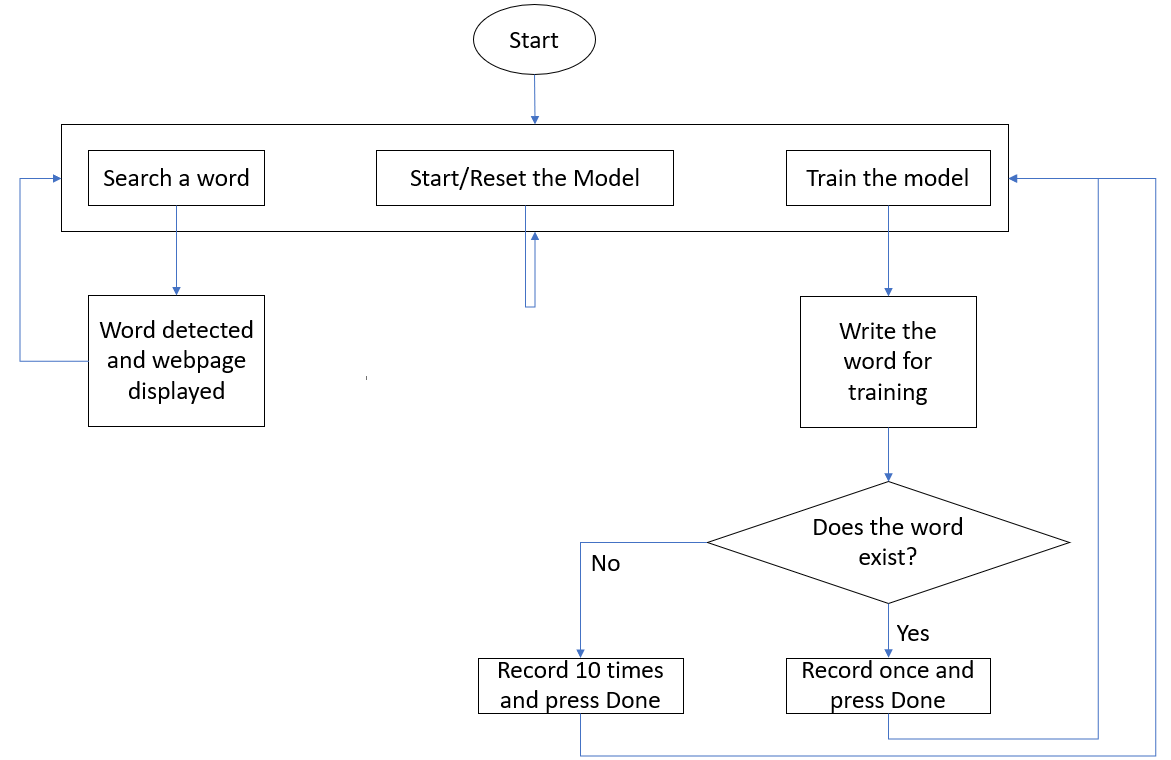
\includegraphics[scale=0.6]{flowchart.png}
\caption{Flowchart of the project}
\label{fig:fc}
\end{figure}
\subsection{Model description}
We are using the famous Hidden Markov Model to store the speech properties. Hidden Markov Model is a probabilistic model which is used to explain or derive the probabilistic characteristic of any random process. When we apply log function to the spectral representation of the speech during reverse fourier transform, it is converted to cepstrum whose coefficients are steady because of application of log function and it represents the speech is a nice manner. This representation can be used as the speech property. We take all such cepstral coefficients and build a codebook which helps in generating the observation sequences. Codebook contains $10$ speech samples for each word.\\
We use feed-forward model for modelling speech samples. While speaking, we speak a word from start to end. So, there is no need of backward movement. Also, the stress on current phoneme is more than moving to the next phoneme. Hence we use feed-forward model. Then while testing, we score each model using the forward process and pick the word with highest score as the result.\\
Since, speech signals depend a lot on the environment, live testing might not be very good. But, if we train the model live and test it immediately, then we get significantly better accuracy.

\section{Result}
\begin{figure}

\includegraphics[scale=1.0]{homepage.png}
\caption{Home Page}
\label{fig:hp}
\end{figure}
\begin{figure}

\includegraphics[scale=1.0]{about.png}
\caption{About Section}
\label{fig:about}
\end{figure}
\begin{figure}

\includegraphics[scale=1.0]{searchPage.png}
\caption{Live Training}
\label{fig:train}
\end{figure}
\begin{figure}

\includegraphics[scale=1.0]{existingWord.png}
\caption{Existing Word Search}
\label{fig:searchOld}
\end{figure}
\begin{figure}

\includegraphics[scale=1.0]{newWord.png}
\caption{New Word Search}
\label{fig:searchNew}
\end{figure}
\begin{figure}
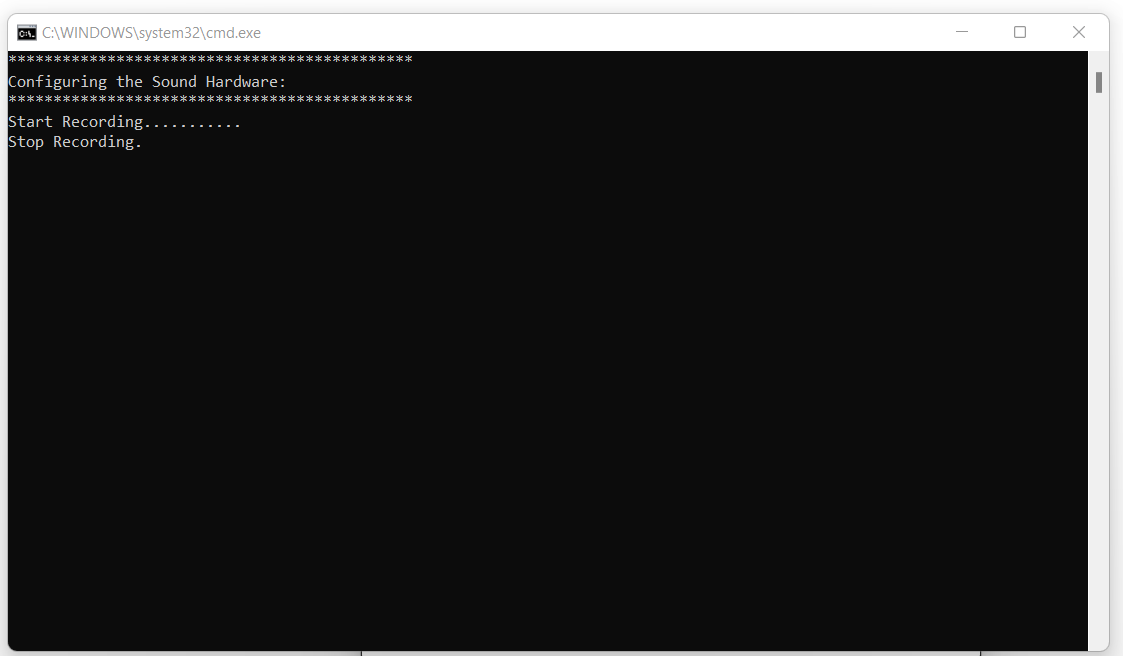
\includegraphics[scale=0.7]{console.png}
\caption{Recording Console}
\label{fig:rc}
\end{figure}
\begin{figure}

\includegraphics[scale=0.6]{wiki.png}
\caption{Display of Webpage}
\label{fig:wp}
\end{figure}

\subsection{Home Page}
Figure ~\ref{fig:hp} shows the homepage of the project. If About button is clicked then Figure ~\ref{fig:about} will be displayed.

\subsection{Live Testing}
For live testing, corresponding button should be clicked. Then recording module will be opened which is showed in Figure ~\ref{fig:rc}. A word can be spoken and recorded for testing. The corresponding webpage will be displayed e.g. Figure ~\ref{fig:wp}.

\subsection{Live Training}
For live training, corresponding button should be clicked. Then Figure ~\ref{fig:train} will be displayed. A word can be entered. It will detect whether the word is already present i.e. Figure ~\ref{fig:searchOld} or new i.e. Figure ~\ref{fig:searchNew}. If the word is already present, then recording will be allowed once, otherwise ten times. For recording, the same Figure ~\ref{fig:rc} will be displayed. After recording, Done button can be clicked to get back to homepage i.e. Figure ~\ref{fig:hp}.

\section{Source Code}
A few files are too large. Hence the entire code is not added here. A few short files are added.
\subsection{commonvar.h}
\begin{lstlisting}

long double *** xi = NULL; //xi in problem-3 solution


long double ** alpha = NULL; //Gets calculated in forward process

long double ** beta = NULL; //Gets calculated in backward process

long double ** delta = NULL; //Gets calculated in Viterbi Algorithm

long double ** gamma = NULL; //Gets calculated in Baum Welch method

long double ** A = NULL; //Transition matrix

long double ** AComplement = NULL; //updated A

long double ** B = NULL; //Probability matrix

long double ** BComplement = NULL; //updated B


long double * Pi = NULL; //Initial probability

long double * PiComplement = NULL; //updated Pi

long double ** codebook = NULL; //codebook

long double pOfOGivenLambda = 0; //probability of an observation sequence given the model lambda

long double pStar = 0; //probability of the state sequence being helpful in modelling

long double pStarComplement = 0; //probability of the state sequence being helpful in modelling for the updated model

long double floorB = 1e-30;


int ** psi = NULL; //Gets generated in Viterbi.h


int * O = NULL; //Observation sequences

int * qStar = NULL; //State sequence

int * qStarComplement = NULL; //State sequence for the updated model

char * resultWord = NULL;

int N = 0; //number of states

int M = 0; //codebook size or number of observations

int T = 100; //size of observation sequence

int R = 0; //read it from file, it will store the number of utterances per word currently present in the universe

int duration = 0; //read it from file, it will store the duration of the recording to be considered

int p = 12; //size of Codebook vectors

int universeSize = 0; //size of the universe

FILE * AComplementFile = NULL; //new A will be printed

FILE * BComplementFile = NULL; //new B will be printed

FILE * PiComplementFile = NULL; //new Pi will be printed

void define()
{
	int i = 0, j = 0;
	delta = new long double *[N];
	psi = new int *[N];
	qStar = new int[T];
	qStarComplement = new int[T];

	for (i = 0; i < N; ++i)
		delta[i] = new long double[T];
	for (i = 0; i < N; ++i)
		psi[i] = new int[T];

	xi = new long double ** [N];
	for (i = 0; i < N; ++i)
		xi[i] = new long double * [N];
	for (i = 0; i < N; ++i)
		for (j = 0; j < N; ++j)
			xi[i][j] = new long double[T-1];

	gamma = new long double * [N];
	for (i = 0; i < N; ++i)
		gamma[i] = new long double[T];

	PiComplement = new long double [N];

	AComplement = new long double * [N];
	for (i = 0; i < N; ++i)
		AComplement[i] = new long double[N];

	BComplement = new long double * [N];
	for (i = 0; i < N; ++i)
		BComplement[i] = new long double[M];

	O = new int [N]; //Observation Sequence
}

FILE * dataOutputFile = NULL; //output file for required output

FILE * modelOutputFile = NULL; //output file for model	
\end{lstlisting}

% \subsection{lbg.h}
% \begin{lstlisting}
% extern int M, universeSize;
% extern long double ** codebook;
% int K = M;

% void KMeans(char * fileName, int currK, long double delta, long double w[])
% {
% 	int minIndex = 9999999; //minIndex stores the index of the code vector with minimum distortion
% 	/*previous distortion stores the distortion of iteration m-1
% 	current distortion stores the distortion of iteration m
% 	min stores the distortion value of the code vector with minimum distortion
% 	totalDistortion stores the total distortion of the universe*/
% 	long double previousDistortion = 0.0, currentDistortion = 1000.0, min = 1000000000.0, totalDistortion = 0.0, temp = 0;
% 	long long int iterationCount = 0; //total number of iterations in kmeans
% 	/*bucketNumber stores values from 0 to N-1 included i.e. the respective bucket numbers of all the vectors in the universe
% 	bucketSize stores the number of x vectors of each bucket*/
% 	int * bucketNumber = new int[universeSize], * bucketSize = new int[K]; //should lie between 0 to K-1 included
% 	long double * distances = new long double[K]; //stores the tokhura distances
% 	long double ** bucketSum = new long double*[K]; //stores the sum of buckets
% 	long double * currentUniverseVector = new long double[p]; // holds the current universe vector
% 	int i = 0, j = 0, k = 0, m = 0; //loop variables
% 	FILE * file = NULL;

% 	//initialize everything to 0
% 	for (i = 0; i < currK; ++i)
% 		bucketSum[i] = new long double[p];
% 	for (i = 0; i < currK; ++i)
% 		bucketSize[i] = 0;
% 	for (i = 0; i < currK; ++i)
% 		for (j = 0; j < p; ++j)
% 			bucketSum[i][j] = 0;
	
% 	i = 0;
% 	j = 0;
% 	while (abs(currentDistortion-previousDistortion) >= delta) //till the difference is more than the threshold
% 	{
% 	++iterationCount;
% 	totalDistortion = 0;
% 	for (i = 0; i < currK; ++i)
% 		bucketSize[i] = 0;
% 	for (i = 0; i < currK; ++i)
% 		for (j = 0; j < p; ++j)
% 			bucketSum[i][j] = 0;
% 	file = fopen(fileName,"r");
% 	//////////////////////////////////////////////////////////////////////////////////////////////////////////////////////////////
% 	/*classification*/
% 	for (i = 0; i < universeSize; ++i) //for each vector in the universe
% 	{
% 		//read the current vector from the file
% 		for (j = 0; j < p; ++j) //for each value in current row of the file
% 		{
% 			fscanf(file,"\%lf",&temp); //read the next value
% 			currentUniverseVector[j] = temp; //add it to the corresponding index of the current universe vector
% 		}

% 		min = 1000000000.0; //reset the minimum

% 		//find out the tokhura distances from each vector in the codebook
% 		for (j = 0; j < currK; ++j) //for each vector in the codebook
% 		{
% 			distances[j] = 0;
% 			for (k = 0; k < p; ++k) //for each p value
% 			{
% 				distances[j] += w[k]*(currentUniverseVector[k]-codebook[j][k])*(currentUniverseVector[k]-codebook[j][k]); //find out the distance
% 			}
% 		}

% 		//find out the minimum
% 		for (j = 0; j < currK; ++j)
% 		{
% 			if (min > distances[j])
% 			{
% 				min = distances[j];
% 				minIndex = j;
% 			}
% 		}

% 		//store the minIndex in the bucketNumber array
% 		bucketNumber[i] = minIndex;

% 		//increase the corresponding bucket size
% 		++bucketSize[minIndex];

% 		/*//update the maximum bucket size
% 		if (bucketSize[minIndex] > M)
% 			M = bucketSize[minIndex];*/

% 		//add the current vector to the bucket sum
% 		for (j = 0; j < p; ++j)
% 			bucketSum[minIndex][j] += currentUniverseVector[j];

% 		//add the current distortion to the distortion sum
% 		totalDistortion += min;
% 	}

% 	//////////////////////////////////////////////////////////////////////////////////////////////////////////////////////////////
% 	/*code vector updation*/

% 	//taking the average and updating the codebook
% 	for (i = 0; i < currK; ++i)
% 		for (j = 0; j < p; ++j)
% 			codebook[i][j] = bucketSum[i][j]/bucketSize[i];

% 	previousDistortion = currentDistortion; //store the previous distortion
% 	currentDistortion = totalDistortion / universeSize; //find out the current distortion
% 	fclose(file);
% 	}
% 	delete(bucketNumber);
% 	delete(bucketSize);
% 	delete(distances);
% 	delete(bucketSum);
% 	delete(currentUniverseVector);
% }

% void LBG(char * fileName, long double * initialCodebook, long double delta, long double epsilon, long double w[])
% {
% 	long double ** tempCodebook = NULL;
% 	codebook = NULL;
% 	int codebookSize = 1;
% 	int i = 0, j = 0, progressCount = 0, printGap = 0, percentageSize = 0;

% 	codebook = new long double*[1];
% 	for (i = 0; i < 1; ++i)
% 		codebook[i] = new long double[p];

% 	//store the initial codebook in codebook
% 	for (i = 0; i < 1; ++i)
% 		for (j = 0; j < p; ++j)
% 			codebook[i][j] = initialCodebook[j];
	
% 	//find out the progress printing details
% 	while(codebookSize != K)
% 	{
% 		codebookSize *= 2;
% 		++printGap;
% 	}
% 	percentageSize = 100/printGap;

% 	codebookSize = 1;
	
% 	printf("\n");
% 	while(codebookSize != K) //till the desired size is not reached
% 	{
% 		tempCodebook = new long double*[2*codebookSize]; //create a double sized codebook
% 		for (j = 0; j < 2*codebookSize; ++j)
% 			tempCodebook[j] = new long double[p];

% 		//split
% 		for (i = 0; i < codebookSize; ++i)
% 		{
% 			for (j = 0; j < p; ++j)
% 			{
% 				tempCodebook[2*i][j] = codebook[i][j]*(1+epsilon);
% 				tempCodebook[(2*i)+1][j] = codebook[i][j]*(1-epsilon);
% 			}
% 		}

% 		codebook = tempCodebook; //store the new codebook
% 		codebookSize *= 2; //update the new codebook size
% 		KMeans(fileName, codebookSize, delta, w); //run k means for optimal codebook

% 		//printing the progress bar
% 		progressCount += percentageSize;
% 		printf("\r"); //move to the beginning of the line
% 		/*print the progress*/
% 		i = 0;
% 		printf("[");
% 		for (i = 1; i <= progressCount; ++i)
% 			printf("|");
% 		for (; i <= 100; ++i)
% 			printf(" ");
% 		printf("]\%d",(progressCount)); //print the percentage
% 	}
% 	//printing the progress bar if it is still incomplete
% 	printf("\r"); //move to the beginning of the line
% 	/*print the progress*/
% 	i = 0;
% 	printf("[");
% 	for (i = 1; i <= 100; ++i)
% 		printf("|");
% 	printf("]\%d",100); //print the percentage
% 	//delete(tempCodebook);
% }

% long double * getInitialCodebook(char * fileName, int rowSize)
% {
% 	FILE * file = NULL;
% 	char * buffer = new char[rowSize];
% 	int i = 0, j = 0;
% 	long double temp = 0;

% 	long double * initialCodebook = new long double[p];

% 	//store 0 in the entire codebook
% 	for (j = 0; j < p; ++j)
% 		initialCodebook[j] = 0;

% 	//add all the vectors from the universe file
% 	file = fopen(fileName,"r");

% 	for (i = 0; i < universeSize; ++i)
% 	{
% 		for (j = 0; j < p; ++j)
% 		{
% 			fscanf(file,"\%lf",&temp); //read the next value
% 			initialCodebook[j] += temp; //add it to the corresponding index of the initial codebook
% 		}
% 	}

% 	fclose(file);

% 	//take the average
% 	for (j = 0; j < p; ++j)
% 		initialCodebook[j] /= universeSize;

% 	delete(buffer);
% 	return initialCodebook;
% }

% void buildCodebook()
% {
% 	/////////////////////////////////////////////////////////////////////////////////////////////////////////////////////////////////////////////////////
% 	/*variable declaration*/
% 	char * universeFileName = "data/universe.txt"; //universe file name
% 	/*universeSize is the total number of vectors given
% 	p stores the value of p
% 	rowSize stores the size of one row of the .csv file
% 	K is the codebook size
% 	*/
% 	int p = 12, rowSize = 1024;
% 	K = M;
% 	long double epsilon = 0.03, delta = 0.00001; // or 0.0001
% 	long double w[] = {1.0,3.0,7.0,13.0,19.0,22.0,25.0,33.0,42.0,50.0,56.0,61.0}; //given Tokhura weights

% 	long double * initialCodebook = NULL;
% 	int i = 0, j = 0; //loop variables

% 	/////////////////////////////////////////////////////////////////////////////////////////////////////////////////////////////////////////////////////
% 	/*execution*/
% 	initialCodebook = getInitialCodebook(universeFileName, rowSize); //generate initial codebook	
% 	LBG(universeFileName, initialCodebook, delta, epsilon, w); //run LBG
% 	FILE * codebookFile = fopen("data/codebook.txt","w+");
% 	for (i = 0; i < M; ++i)
% 	{
% 		for (j = 0; j < p; ++j)
% 			fprintf(codebookFile,"\%lf ",codebook[i][j]);
% 		fprintf(codebookFile,"\n");
% 	}
% 	fclose(codebookFile);
% 	//delete(codebook);
% 	//delete(universeFileName);
% 	//delete(initialCodebook);
% }
% \end{lstlisting}

% \subsection{functions.h}
% \begin{lstlisting}
% extern FILE * AComplementFile, * BComplementFile, * PiComplementFile;
% extern long double pStar, pStarComplement, pOfOGivenLambda;
% extern long double ** AComplement, ** BComplement, ** A, ** B, ** codebook;
% extern long double * PiComplement, * Pi;
% extern int * O;
% extern int N, M, T, duration, p, universeSize;
% extern char * resultWord;

% int noOfFrames = 100, samplingRate = 16000;

% double * getRValues(double * x, int sampleSize, int p)
% {
% 	double * R = new double[13];
% 	int i = 0, j = 0;
% 	for (i = 0; i <= p; ++i)
% 	{
% 		R[i] = 0;
% 		for (j = 0; j < sampleSize-i; ++j)
% 			R[i] += x[j]*x[i+j];
% 	}
% 	return R;
% }

% double * getAValues(double * R, int sampleSize, int p)
% {
% 	//following Durbin's Algorithm
% 	int i = 0, j = 0;
% 	double * AA = new double[p];
% 	double * E = new double[p+1];
% 	double * K = new double[p+1];
% 	double ** tempA = new double*[p+1];

% 	//initializing everything to 0
% 	for (i = 0; i < p+1; ++i)
% 		tempA[i] = new double[p+1];
% 	for (i = 0; i < p+1; ++i)
% 	{
% 		E[i] = 0;
% 		K[i] = 0;
% 	}
% 	for (i = 0; i < p+1; ++i)
% 		for (j = 0; j < p+1; ++j)
% 			tempA[i][j] = 0;

% 	//Algorithm steps
% 	E[0] = R[0];
% 	for (i = 1; i <= p; ++i)
% 	{
% 		K[i] = 0;
% 		for (j = 1; j < i; ++j)
% 			K[i] += tempA[i-1][j]*R[i-j];
% 		K[i] = R[i]-K[i];
% 		K[i] /= E[i-1];
% 		tempA[i][i] = K[i];
% 		for (j = 1; j < i; ++j)
% 			tempA[i][j] = tempA[i-1][j]-(K[i]*tempA[i-1][i-j]);
% 		E[i] = (1-(K[i]*K[i]))*E[i-1];
% 	}
% 	for (i = 1; i <= p; ++i)
% 		AA[i-1] = tempA[p][i];
% 	return AA;
% }

% double * getCValues(double * AA, int sampleSize, int p, double r0)
% {
% 	int i = 0, j = 0;
% 	double * C = new double[p+1];
% 	C[0] = log(r0*r0);
% 	for (i = 1; i < p+1; ++i)
% 	{
% 		C[i] = 0;
% 		double m = i;
% 		for (j = 1; j < i; ++j)
% 		{
% 			double k = j;
% 			C[i] += (k/m)*C[j]*AA[i-j-1];
% 		}
% 		C[i] += AA[i-1];
% 	}
% 	return C;
% }

% void buildUniverse(char * folder, char * digits[], char * files[], int D, int R, int range)
% {
% 	int d = 0, f = 0, r = 0, i = 0, j = 0, k = 0, q = p, index = 0, prog = 0;
% 	int xCount = duration*samplingRate, dcCount = 0, shift = 0, temp = 0, sampleSize = xCount/noOfFrames;
% 	char * buffer = new char[1024];
% 	double * x = new double[xCount], * RR = NULL, * AA = NULL, * C = NULL, * trainingData = new double[sampleSize];
% 	double DCShift = 0, maxData = 0, minData = 0, normalizationFactor = 0, copy = 0;
% 	char fileName[100];
% 	FILE * universeFile = fopen("data/universe.txt","w+"), * file = NULL;

% 	/////////////////////////////////////////////////////////////////
% 	//Implementing a progress bar
% 	int nop = D*R*noOfFrames;
% 	int percentageBreak = D*R;
% 	int progressCount = 0;
% 	/////////////////////////////////////////////////////////////////
% 	printf("\n");
% 	for (d = 0; d < D; ++d)
% 	{		
% 		for (f = 0; f < R; ++f)
% 		{
% 			sprintf(fileName,"\%s\%s/\%s.txt",folder,digits[d],files[f]);

% 			file = fopen(fileName,"r");
% 			dcCount = 0;
% 			for (i = 0; i < 1000; ++i) //for all x values
% 			{
% 				fgets(buffer, 1024, file); //read one line from the file
% 				x[i] = atof(buffer); //convert it into float
% 				DCShift += x[i]; ++dcCount; //add it to dc shift
% 			}
% 			DCShift /= dcCount; //find out dcshift
% 			for (i = 0; i < 1000; ++i)
% 			{
% 				x[i] -= DCShift; //subtract dcshift from already stored values
% 				if (x[i] > maxData) maxData = x[i]; //update maxData
% 				if (x[i] < minData) minData = x[i]; //update minData
% 			}
% 			for (i = 1000; i < xCount; ++i) //for rest values
% 			{
% 				fgets(buffer, 1024, file); //read one line from the file
% 				x[i] = atof(buffer); //convert it into float
% 				x[i] -= DCShift; //subtract dcshift
% 				if (x[i] > maxData) maxData = x[i]; //update maxData
% 				if (x[i] < minData) minData = x[i]; //update minData
% 			}
% 			fclose(file);

% 			//find out normalization factor
% 			minData = abs(minData); //get the absolute value of the minimum
% 			normalizationFactor = range/((maxData+minData)/2); //get the normalization factor
% 			//truncate the normalizationFactor to one decimal digit
% 			copy = normalizationFactor; //store the normalizationFactor in copy
% 			while (copy < 1) //till copy is less than 1
% 			{
% 				++shift; //increment shift
% 				copy *= 10; //keep multiplying copy with 10
% 			}
% 			temp = (int)copy; //store the integer part of copy in temp
% 			copy -= temp; //subtract temp from copy
% 			while (shift-- > 0) //reverse the shift process
% 				copy /= 10;
% 			/*the above process helps in getting all the digits except the first decimal digit*/
% 			normalizationFactor -= copy; //subtract copy from normalizationFactor
% 			/*this will ensure that only one digit remains after decimal point*/

% 			//multiply normalization factor
% 			for (i = 0; i < xCount; ++i)
% 				x[i] *= normalizationFactor;

% 			index = 0;

% 			for (r = 0; r < noOfFrames; ++r) //indicates frame number
% 			{
% 				for (i = 0; i < sampleSize; ++i)
% 					trainingData[i] = x[index++];

% 				RR = getRValues(trainingData,sampleSize,p);
% 				AA = getAValues(RR,sampleSize,p);
% 				C = getCValues(AA,sampleSize,p,RR[0]);
				
% 				//raised sine window on C and adding it to the universe file
% 				for (j = 1; j <= p; ++j)
% 				{
% 					C[j] *= 1+((q/2)*sin((3.14*j)/q));
% 					fprintf(universeFile,"\%f ",C[j]);
% 				}
% 				++universeSize;
% 				fprintf(universeFile,"\n");
				
% 				//printing the progress bar
% 				++progressCount;
% 				if (progressCount\%percentageBreak == 0)
% 				{
% 					printf("\r"); //move to the beginning of the line
% 					/*print the progress*/
% 					prog = 0;
% 					printf("[");
% 					for (prog = percentageBreak; prog <= progressCount; prog += percentageBreak)
% 						printf("|");
% 					for (; prog <= nop; prog += percentageBreak)
% 						printf(" ");
% 					printf("]\%d",(progressCount/percentageBreak)); //print the percentage
% 				}
% 			}
% 		}
% 	}
	
% 	fclose(universeFile);
% 	delete(x);
% 	delete(buffer);
% 	delete(RR);
% 	delete(AA);
% 	delete(C);
% 	delete(trainingData);
% }

% bool compareAndUpdateModel()
% {
% 	int i = 0, j = 0, t = 0, m = 0;
% 	if (pStarComplement > pStar)
% 	//if (pStarComplement < 1e-30)
% 	//if (abs(pStarComplement-pStar) > 1e-2)
% 	{
% 		//update A
% 		for (i = 0; i < N; ++i)
% 			for (j = 0; j < N; ++j)
% 				A[i][j] = AComplement[i][j];
		
% 		//update B
% 		for (i = 0; i < N; ++i)
% 			for (m = 0; m < M; ++m)
% 				B[i][m] = BComplement[i][m];
		
% 		//update Pi
% 		for (j = 0; j < N; ++j)
% 			Pi[j] = PiComplement[j];
	
% 		//update pStar
% 		pStar = pStarComplement;

% 		return true;
% 	}
% 	else
% 	{
% 		return false;
% 	}
% }

% void generateObservationSequences(char * folder, char * digits[], char * files[], int digitIndex, int F, int range)
% {
% 	int f = 0, r = 0, i = 0, j = 0, k = 0, q = p, index = 0, codeBookIndex = 0;
% 	int xCount = duration*samplingRate, dcCount = 0, shift = 0, temp = 0, sampleSize = xCount/noOfFrames, minIndex = -1;
% 	char * buffer = new char[1024];
% 	double * x = new double[xCount], * RR = NULL, * AA = NULL, * C = NULL, * trainingData = new double[sampleSize];
% 	double DCShift = 0, maxData = 0, minData = 0, normalizationFactor = 0, copy = 0;
% 	int ** Ob = new int*[F];
% 	long double * distances = new long double[M]; //stores the tokhura distances
% 	long double w[] = {1.0,3.0,7.0,13.0,19.0,22.0,25.0,33.0,42.0,50.0,56.0,61.0}; //given Tokhura weights
% 	long double min = 1e30, temp1 = 0, temp2 = 0;
% 	char fileName[100];
% 	FILE * file = NULL;
% 	for (i = 0; i < F; ++i)
% 		Ob[i] = new int[noOfFrames];	
% 	for (f = 0; f < F; ++f)
% 	{
% 		sprintf(fileName,"\%s\%s/\%d.txt",folder,digits[digitIndex],f);

% 		file = fopen(fileName,"r");
% 		dcCount = 0;
% 		for (i = 0; i < 1000; ++i) //for all x values
% 		{
% 			fgets(buffer, 1024, file); //read one line from the file
% 			x[i] = atof(buffer); //convert it into float
% 			DCShift += x[i]; ++dcCount; //add it to dc shift
% 		}
% 		DCShift /= dcCount; //find out dcshift
% 		for (i = 0; i < 1000; ++i)
% 		{
% 			x[i] -= DCShift; //subtract dcshift from already stored values
% 			if (x[i] > maxData) maxData = x[i]; //update maxData
% 			if (x[i] < minData) minData = x[i]; //update minData
% 		}
% 		for (i = 1000; i < xCount; ++i) //for rest values
% 		{
% 			fgets(buffer, 1024, file); //read one line from the file
% 			x[i] = atof(buffer); //convert it into float
% 			x[i] -= DCShift; //subtract dcshift
% 			if (x[i] > maxData) maxData = x[i]; //update maxData
% 			if (x[i] < minData) minData = x[i]; //update minData
% 		}
% 		fclose(file);

% 		//find out normalization factor
% 		minData = abs(minData); //get the absolute value of the minimum
% 		normalizationFactor = range/((maxData+minData)/2); //get the normalization factor

% 		//truncate the normalizationFactor to one decimal digit
% 		copy = normalizationFactor; //store the normalizationFactor in copy
% 		while (copy < 1) //till copy is less than 1
% 		{
% 			++shift; //increment shift
% 			copy *= 10; //keep multiplying copy with 10
% 		}
% 		temp = (int)copy; //store the integer part of copy in temp
% 		copy -= temp; //subtract temp from copy
% 		while (shift-- > 0) //reverse the shift process
% 			copy /= 10;
% 		/*the above process helps in getting all the digits except the first decimal digit*/
% 		normalizationFactor -= copy; //subtract copy from normalizationFactor
% 		/*this will ensure that only one digit remains after decimal point*/

% 		//multiply normalization factor
% 		for (i = 0; i < xCount; ++i)
% 			x[i] *= normalizationFactor;

% 		index = 0;
% 		for (r = 0; r < noOfFrames; ++r) //indicates frame number
% 		{
% 			for (i = 0; i < sampleSize; ++i)
% 				trainingData[i] = x[index++];

% 			RR = getRValues(trainingData,sampleSize,p);
% 			AA = getAValues(RR,sampleSize,p);
% 			C = getCValues(AA,sampleSize,p,RR[0]);
			
% 			//raised sine window on C and adding it to the universe file
% 			for (j = 1; j <= p; ++j)
% 				C[j] *= 1+((q/2)*sin((3.14*j)/q));

% 			//Tokhura Distance from codebook
% 			file = fopen("data/codebook.txt","r");
% 			for (j = 0; j < M; ++j) //for each vector in the codebook
% 			{
% 				distances[j] = 0;
% 				for (k = 0; k < p; ++k) //for each p value
% 				{
% 					temp1 = (long double)C[k+1];
% 					fscanf(file,"\%lf",&temp2);
% 					distances[j] += w[k]*(temp1-temp2)*(temp1-temp2); //find out the distance
% 				}
% 			}
% 			fclose(file);
% 			//Minimum index
% 			min = 1e30; //reset the minimum
% 			for (j = 0; j < M; ++j)
% 			{
% 				if (min > distances[j])
% 				{
% 					min = distances[j];
% 					minIndex = j;
% 				}
% 			}

% 			Ob[f][r] = minIndex+1; //+1 is done to maintain the 1-32 range format and not 0-31 since this subtraction is being done at later steps
% 		}
% 	}

% 	sprintf(fileName,"\%s\%s/O.txt",folder,digits[digitIndex]);
% 	file = fopen(fileName,"w+");
% 	for (i = 0; i < F; ++i)
% 	{
% 		for (j = 0; j < noOfFrames; ++j)
% 		{
% 			fprintf(file,"\%d ",Ob[i][j]);
% 		}
% 		fprintf(file,"\n");
% 	}
% 	fclose(file);
% 	delete(x);
% 	delete(buffer);
% 	delete(Ob);
% 	delete(RR);
% 	delete(AA);
% 	delete(C);
% 	delete(trainingData);
% }

% void resetCount(char * folder, char * digits[], char * files[], int D, int R)
% {
% 	int d = 0;
% 	char fileName[100];
% 	FILE * countFile = NULL;
% 	for (d = 0; d < D; ++d)
% 	{
% 		sprintf(fileName,"\%s\%s/count.txt",folder,digits[d]);
% 		countFile = fopen(fileName,"w");

% 		fprintf(countFile,"\%d\n",R);

% 		fclose(countFile);
% 	}
% }

% void resetModel(char * folder, char * digits[], char * files[], int D, int R)
% {
% 	int d = 0, k = 0, i = 0, j = 0;
% 	FILE * AFile = NULL, * BFile = NULL, * PiFile = NULL;
% 	char fileName[100];
% 	long double * row = new long double[N];
% 	long double tempB = 0.03125, one = 1, zero = 0;
% 	row[0] = 0.8;
% 	row[1] = 0.2;
% 	row[2] = row[3] = row[4] = 0;
% 	for (d = 0; d < D; ++d)
% 	{
% 		sprintf(fileName,"\%s\%s/A.txt",folder,digits[d]);
% 		AFile = fopen(fileName,"w");

% 		sprintf(fileName,"\%s\%s/B.txt",folder,digits[d]);
% 		BFile = fopen(fileName,"w");

% 		sprintf(fileName,"\%s\%s/Pi.txt",folder,digits[d]);
% 		PiFile = fopen(fileName,"w");

% 		tempB = 0.03125, one = 1, zero = 0;
% 		row[0] = 0.8;
% 		row[1] = 0.2;
% 		row[2] = row[3] = row[4] = 0;

% 		for (i = 0; i < N-1; ++i)
% 		{
% 			for (j = 0; j < N; ++j)
% 				fprintf(AFile,"\%g ",row[j]);
% 			fprintf(AFile,"\n");
% 			for (j = N-2; j >= 0; --j)
% 				row[j+1] = row[j];
% 			row[0] = 0;
% 		}
% 		for (i = 0; i < N-1; ++i)
% 			fprintf(AFile,"\%g ",zero);
% 		fprintf(AFile,"\%g \n",one);

% 		for (i = 0; i < N; ++i)
% 		{
% 			for (j = 0; j < M; ++j)
% 				fprintf(BFile,"\%g ",tempB);
% 			fprintf(BFile,"\n");
% 		}

% 		fprintf(PiFile,"\%g ",one);
% 		for (i = 1; i < N; ++i)
% 			fprintf(PiFile,"\%g ",zero);
% 		fprintf(PiFile,"\n");

% 		fclose(AFile);
% 		fclose(BFile);
% 		fclose(PiFile);
% 	}
% }

% void recognize(char * folder, char * digits[], char * files[], char * dataFiles[], int D, int R, int range, char * testFileName)
% {
% 	int d = 0, f = 0, r = 0, i = 0, j = 0, k = 0, q = p, index = 0;
% 	int xCount = duration*samplingRate, dcCount = 0, shift = 0, temp = 0, sampleSize = xCount/noOfFrames, minIndex = -1;
% 	char * buffer = new char[1024];
% 	double * x = new double[xCount], * RR = NULL, * AA = NULL, * C = NULL, * trainingData = new double[sampleSize];
% 	double DCShift = 0, maxData = 0, minData = 0, normalizationFactor = 0, copy = 0;
% 	int * Ob = new int[noOfFrames];
% 	long double * distances = new long double[M]; //stores the tokhura distances
% 	long double w[] = {1.0,3.0,7.0,13.0,19.0,22.0,25.0,33.0,42.0,50.0,56.0,61.0}; //given Tokhura weights
% 	long double min = 1e30, temp1 = 0, temp2 = 0, maxProb = 0;
% 	char fileName[200], * resultantWord = NULL;
% 	FILE * file = NULL, * AFile = NULL, * BFile = NULL, * PiFile = NULL;	

% 	printf("\%s\n",testFileName);
% 	file = fopen(testFileName,"r");
% 	dcCount = 0;
% 	for (i = 0; i < 1000; ++i) //for all x values
% 	{
% 		fgets(buffer, 1024, file); //read one line from the file
% 		x[i] = atof(buffer); //convert it into float
% 		DCShift += x[i]; ++dcCount; //add it to dc shift
% 	}
% 	DCShift /= dcCount; //find out dcshift
% 	for (i = 0; i < 1000; ++i)
% 	{
% 		x[i] -= DCShift; //subtract dcshift from already stored values
% 		if (x[i] > maxData) maxData = x[i]; //update maxData
% 		if (x[i] < minData) minData = x[i]; //update minData
% 	}
% 	for (i = 1000; i < xCount; ++i) //for rest values
% 	{
% 		fgets(buffer, 1024, file); //read one line from the file
% 		x[i] = atof(buffer); //convert it into float
% 		x[i] -= DCShift; //subtract dcshift
% 		if (x[i] > maxData) maxData = x[i]; //update maxData
% 		if (x[i] < minData) minData = x[i]; //update minData
% 	}
% 	fclose(file);

% 	//find out normalization factor
% 	minData = abs(minData); //get the absolute value of the minimum
% 	normalizationFactor = range/((maxData+minData)/2); //get the normalization factor

% 	//truncate the normalizationFactor to one decimal digit
% 	copy = normalizationFactor; //store the normalizationFactor in copy
% 	while (copy < 1) //till copy is less than 1
% 	{
% 		++shift; //increment shift
% 		copy *= 10; //keep multiplying copy with 10
% 	}
% 	temp = (int)copy; //store the integer part of copy in temp
% 	copy -= temp; //subtract temp from copy
% 	while (shift-- > 0) //reverse the shift process
% 		copy /= 10;
% 	/*the above process helps in getting all the digits except the first decimal digit*/
% 	normalizationFactor -= copy; //subtract copy from normalizationFactor
% 	/*this will ensure that only one digit remains after decimal point*/

% 	//multiply normalization factor
% 	for (i = 0; i < xCount; ++i)
% 		x[i] *= normalizationFactor;
	
% 	index = 0;
	
% 	for (r = 0; r < noOfFrames; ++r) //indicates frame number
% 	{
% 		for (i = 0; i < sampleSize; ++i) //copy the next frame to training data
% 			trainingData[i] = x[index++];

% 		//find out Ci
% 		RR = getRValues(trainingData,sampleSize,p);
% 		AA = getAValues(RR,sampleSize,p);
% 		C = getCValues(AA,sampleSize,p,RR[0]);
			
% 		//raised sine window on C and adding it to the universe file
% 		for (j = 1; j <= p; ++j)
% 			C[j] *= 1+((q/2)*sin((3.14*j)/q));

% 		//Tokhura Distance from codebook
% 		file = fopen("data/codebook.txt","r");
% 		for (j = 0; j < M; ++j) //for each vector in the codebook
% 		{
% 			distances[j] = 0;
% 			for (k = 0; k < p; ++k) //for each p value
% 			{
% 				temp1 = (long double)C[k+1];
% 				fscanf(file,"\%lf",&temp2);
% 				distances[j] += w[k]*(temp1-temp2)*(temp1-temp2); //find out the distance
% 			}
% 		}
		
% 		fclose(file);
% 		//Minimum index
% 		min = 1e30; //reset the minimum
% 		for (j = 0; j < M; ++j)
% 		{
% 			if (min > distances[j])
% 			{
% 				min = distances[j];
% 				minIndex = j;
% 			}
% 		}

% 		Ob[r] = minIndex+1; //+1 is done to maintain the 1-32 range format and not 0-31 since this subtraction is being done at later steps
% 	}

% 	O = Ob;
% 	for (d = 0; d < D; ++d)
% 	{
% 		strcpy(fileName,folder);
% 		strcat(fileName,digits[d]);
% 		strcat(fileName,"/A.txt");
% 		AFile = fopen(fileName,"r");
% 		strcpy(fileName,folder);
% 		strcat(fileName,digits[d]);
% 		strcat(fileName,"/B.txt");
% 		BFile = fopen(fileName,"r");
% 		strcpy(fileName,folder);
% 		strcat(fileName,digits[d]);
% 		strcat(fileName,"/Pi.txt");
% 		PiFile = fopen(fileName,"r");

% 		for (i = 0; i < N; ++i)
% 			for (j = 0; j < N; ++j)
% 				fscanf(AFile,"\%lf",&A[i][j]);

% 		for (i = 0; i < N; ++i)
% 			for (j = 0; j < M; ++j)
% 				fscanf(BFile,"\%lf",&B[i][j]);

% 		for (i = 0; i < N; ++i)
% 			fscanf(PiFile,"\%lf",&Pi[i]);

% 		runForwardBackward();

% 		printf("d = \%s, \%g\n",digits[d],pOfOGivenLambda);
% 		if (pOfOGivenLambda > maxProb)
% 		{
% 			maxProb = pOfOGivenLambda;
% 			resultantWord = digits[d];
% 		}

% 		fclose(AFile);
% 		fclose(BFile);
% 		fclose(PiFile);
% 	}

% 	delete(x);
% 	delete(buffer);
% 	delete(Ob);
% 	delete(RR);
% 	delete(AA);
% 	delete(C);
% 	delete(trainingData);
% 	resultWord = resultantWord;
% }

% void trainModel(char * word, int range, char * trainFileName)
% {
% 	bool isUpdated = true;
% 	int xCount = duration*samplingRate, dcCount = 0, shift = 0, temp = 0, q = p, sampleSize = xCount/noOfFrames, minIndex = -1, index = 0, codebookIndex = 0, updationLimit = 0, currCount = -1;
% 	char * buffer = new char[1024];
% 	double * x = new double[xCount], * RR = NULL, * AA = NULL, * C = NULL, * trainingData = new double[sampleSize];
% 	double DCShift = 0, maxData = 0, minData = 0, normalizationFactor = 0, copy = 0;
% 	O = new int[noOfFrames];
% 	long double * distances = new long double[M]; //stores the tokhura distances
% 	long double w[] = {1.0,3.0,7.0,13.0,19.0,22.0,25.0,33.0,42.0,50.0,56.0,61.0}; //given Tokhura weights
% 	long double min = 1e30, temp1 = 0, temp2 = 0, tempValue = 0;
% 	FILE * file = NULL;
	
% 	int i = 0, j = 0, r = 0, k = 0, m = 0;
% 	char filePath[128];
% 	sprintf(filePath,"HMM/\%s/",word);
% 	char fileName[256];

% 	//define variables
% 	define();

% 	//set A B and Pi to Bakis model
% 	long double * row = new long double[N];
% 	long double tempB = 0.03125, one = 1, zero = 0;
% 	row[0] = 0.8;
% 	row[1] = 0.2;
% 	row[2] = row[3] = row[4] = 0;

% 	for (i = 0; i < N-1; ++i)
% 	{
% 		for (j = 0; j < N; ++j)
% 			A[i][j] = row[j];
% 		for (j = N-2; j >= 0; --j)
% 			row[j+1] = row[j];
% 		row[0] = 0;
% 	}
% 	for (i = 0; i < N-1; ++i)
% 		A[N-1][i] = zero;
% 	A[N-1][N-1] = one;

% 	for (i = 0; i < N; ++i)
% 	{
% 		for (j = 0; j < M; ++j)
% 			B[i][j] = tempB;
% 	}

% 	Pi[0] = 1;
% 	for (i = 1; i < N; ++i)
% 		Pi[i] = 0;

% 	//generate observation sequence for the spoken word
% 	file = fopen(trainFileName,"r");
% 	dcCount = 0;
% 	for (i = 0; i < 1000; ++i) //for all x values
% 	{
% 		fgets(buffer, 1024, file); //read one line from the file
% 		x[i] = atof(buffer); //convert it into float
% 		DCShift += x[i]; ++dcCount; //add it to dc shift
% 	}
% 	DCShift /= dcCount; //find out dcshift
% 	for (i = 0; i < 1000; ++i)
% 	{
% 		x[i] -= DCShift; //subtract dcshift from already stored values
% 		if (x[i] > maxData) maxData = x[i]; //update maxData
% 		if (x[i] < minData) minData = x[i]; //update minData
% 	}
% 	for (i = 1000; i < xCount; ++i) //for rest values
% 	{
% 		fgets(buffer, 1024, file); //read one line from the file
% 		x[i] = atof(buffer); //convert it into float
% 		x[i] -= DCShift; //subtract dcshift
% 		if (x[i] > maxData) maxData = x[i]; //update maxData
% 		if (x[i] < minData) minData = x[i]; //update minData
% 	}
% 	fclose(file);

% 	//find out normalization factor
% 	minData = abs(minData); //get the absolute value of the minimum
% 	normalizationFactor = range/((maxData+minData)/2); //get the normalization factor

% 	//truncate the normalizationFactor to one decimal digit
% 	copy = normalizationFactor; //store the normalizationFactor in copy
% 	while (copy < 1) //till copy is less than 1
% 	{
% 		++shift; //increment shift
% 		copy *= 10; //keep multiplying copy with 10
% 	}
% 	temp = (int)copy; //store the integer part of copy in temp
% 	copy -= temp; //subtract temp from copy
% 	while (shift-- > 0) //reverse the shift process
% 		copy /= 10;
% 	/*the above process helps in getting all the digits except the first decimal digit*/
% 	normalizationFactor -= copy; //subtract copy from normalizationFactor
% 	/*this will ensure that only one digit remains after decimal point*/

% 	//multiply normalization factor
% 	for (i = 0; i < xCount; ++i)
% 		x[i] *= normalizationFactor;

% 	index = 0;
% 	for (r = 0; r < noOfFrames; ++r) //indicates frame number
% 	{
% 		for (i = 0; i < sampleSize; ++i)
% 			trainingData[i] = x[index++];

% 		RR = getRValues(trainingData,sampleSize,p);
% 		AA = getAValues(RR,sampleSize,p);
% 		C = getCValues(AA,sampleSize,p,RR[0]);
			
% 		//raised sine window on C and adding it to the universe file
% 		for (j = 1; j <= p; ++j)
% 			C[j] *= 1+((q/2)*sin((3.14*j)/q));

% 		//Tokhura Distance from codebook
% 		file = fopen("data/codebook.txt","r");
% 		for (j = 0; j < M; ++j) //for each vector in the codebook
% 		{
% 			distances[j] = 0;
% 			for (k = 0; k < p; ++k) //for each p value
% 			{
% 				temp1 = (long double)C[k+1];
% 				fscanf(file,"\%lf",&temp2);
% 				distances[j] += w[k]*(temp1-temp2)*(temp1-temp2); //find out the distance
% 			}
% 		}
% 		fclose(file);
% 		//Minimum index
% 		min = 1e30; //reset the minimum
% 		for (j = 0; j < M; ++j)
% 		{
% 			if (min > distances[j])
% 			{
% 				min = distances[j];
% 				minIndex = j;
% 			}
% 		}

% 		O[r] = minIndex+1; //+1 is done to maintain the 1-32 range format and not 0-31 since this subtraction is being done at later steps
% 	}

% 	//train the model
% 	isUpdated = true;

% 	//update new pStar
% 	runViterbi(0);
% 	updationLimit = 0;

% 	//run till the model is being updated
% 	while(isUpdated && updationLimit++ <= 200)
% 	{
% 		runForwardBackward();
% 		runBaumWelch();
% 		runViterbi(1);
% 		isUpdated = compareAndUpdateModel();
% 	}
			
% 	//print the new models to respective files
% 	strcpy(fileName,filePath);
% 	strcat(fileName,"count.txt");
% 	file = fopen(fileName,"r");
% 	fscanf(file,"\%d",&currCount);
% 	fclose(file);

% 	file = fopen(fileName,"w");
% 	fprintf(file,"\%d\n",(currCount+1));
% 	fclose(file);

% 	strcpy(fileName,filePath);
% 	strcat(fileName,"A.txt");

% 	file = fopen(fileName,"r");

% 	for (i = 0; i < N; ++i)
% 		for (j = 0; j < N; ++j)
% 			fscanf(file,"\%lf",&AComplement[i][j]);

% 	fclose(file);

% 	file = fopen(fileName,"w");

% 	for (i = 0; i < N; ++i)
% 	{
% 		for (j = 0; j < N; ++j)
% 		{
% 			tempValue = ((currCount*AComplement[i][j])+A[i][j])/(currCount+1);
% 			fprintf(file,"\%g ",tempValue);
% 		}
% 		fprintf(file,"\n");
% 	}
% 	fclose(file);
			
% 	strcpy(fileName,filePath);
% 	strcat(fileName,"B.txt");
	
% 	file = fopen(fileName,"r");

% 	for (i = 0; i < N; ++i)
% 		for (j = 0; j < M; ++j)
% 			fscanf(file,"\%lf",&BComplement[i][j]);

% 	fclose(file);

% 	file = fopen(fileName,"w");

% 	for (i = 0; i < N; ++i)
% 	{
% 		for (m = 0; m < M; ++m)
% 		{
% 			tempValue = ((currCount*BComplement[i][m])+B[i][m])/(currCount+1);
% 			fprintf(file,"\%g ",tempValue);
% 		}
% 		fprintf(file,"\n");
% 	}
% 	fclose(file);
			
% 	strcpy(fileName,filePath);
% 	strcat(fileName,"Pi.txt");

% 	file = fopen(fileName,"r");

% 	for (i = 0; i < N; ++i)
% 		fscanf(file,"\%lf",&PiComplement[i]);

% 	fclose(file);

% 	file = fopen(fileName,"w");

% 	for (j = 0; j < N; ++j)
% 	{
% 		tempValue = ((currCount*PiComplement[j])+Pi[j])/(currCount+1);
% 		fprintf(file,"\%g ",tempValue);
% 	}
% 	fprintf(file,"\n");
% 	fclose(file);
% }

% void writeGeneralModel(char * filePath, int R)
% {
% 	char fileName[256];
% 	FILE * file = NULL;
% 	int d = 0, k = 0, i = 0, j = 0;
% 	long double * row = new long double[N];
% 	long double tempB = 0.03125, one = 1, zero = 0;
% 	row[0] = 0.8;
% 	row[1] = 0.2;
% 	row[2] = row[3] = row[4] = 0;

% 	sprintf(fileName,"\%s/A.txt",filePath);
% 	file = fopen(fileName,"w");

% 	for (i = 0; i < N-1; ++i)
% 	{
% 		for (j = 0; j < N; ++j)
% 			fprintf(file,"\%g ",row[j]);
% 		fprintf(file,"\n");
% 		for (j = N-2; j >= 0; --j)
% 			row[j+1] = row[j];
% 		row[0] = 0;
% 	}
% 	for (i = 0; i < N-1; ++i)
% 		fprintf(file,"\%g ",zero);
% 	fprintf(file,"\%g \n",one);

% 	fclose(file);

% 	sprintf(fileName,"\%s/B.txt",filePath);
% 	file = fopen(fileName,"w");

% 	for (i = 0; i < N; ++i)
% 	{
% 		for (j = 0; j < M; ++j)
% 			fprintf(file,"\%g ",tempB);
% 		fprintf(file,"\n");
% 	}

% 	fclose(file);

% 	sprintf(fileName,"\%s/Pi.txt",filePath);
% 	file = fopen(fileName,"w");

% 	fprintf(file,"\%g ",one);
% 	for (i = 1; i < N; ++i)
% 		fprintf(file,"\%g ",zero);
% 	fprintf(file,"\n");

% 	fclose(file);

% 	sprintf(fileName,"\%s/count.txt",filePath);
% 	file = fopen(fileName,"w");
% 	fprintf(file,"\%d\n",R);
% 	fclose(file);
% }
% \end{lstlisting}

% \subsection{forwardbackward.h}
% \begin{lstlisting}
% extern long double ** A, ** B, ** alpha, ** beta;
% extern long double * Pi;
% extern long double pOfOGivenLambda;
% extern int * O;
% extern int N, M, T;
% extern FILE * dataOutputFile, * modelOutputFile;

% void runForwardBackward()
% {
% 	int i = 0, j = 0, t = 0;

% 	//initialization
% 	for (i = 0; i < N; ++i)
% 		alpha[i][0] = Pi[i]*B[i][O[0]-1];

% 	//induction
% 	for (t = 0; t < T-1; ++t)
% 	{
% 		for (j = 0; j < N; ++j)
% 		{
% 			alpha[j][t+1] = 0;
% 			for (i = 0; i < N; ++i)
% 				alpha[j][t+1] += alpha[i][t]*A[i][j];
% 			alpha[j][t+1] *= B[j][O[t+1]-1];
% 		}
% 	}

% 	//finding out probability
% 	pOfOGivenLambda = 0;
% 	for (i = 0; i < N; ++i)
% 		pOfOGivenLambda += alpha[i][T-1];

% 	//initialization
% 	for (i = 0; i < N; ++i)
% 		beta[i][T-1] = 1;

% 	//induction
% 	for (t = T-2; t >= 0; --t)
% 	{
% 		for (i = 0; i < N; ++i)
% 		{
% 			beta[i][t] = 0;
% 			for (j = 0; j < N; ++j)
% 				beta[i][t] += A[i][j]*B[j][O[t+1]-1]*beta[j][t+1];
% 		}
% 	}
% }
% \end{lstlisting}

% \subsection{viterbi.h}
% \begin{lstlisting}
% extern long double ** A, ** B, ** AComplement, **BComplement, ** delta;
% extern long double * Pi, * PiComplement;
% extern long double pStar, pStarComplement;
% extern int * O, ** psi;
% extern int * qStar, * qStarComplement;
% extern int N, M, T;
% extern FILE * dataOutputFile, * modelOutputFile;

% long double temp = 0;

% void runViterbi(int status)
% {
% 	int i = 0, j = 0, t = 0;
	
% 	if (status == 0)
% 	{
% 		//initialization
% 		for (i = 0; i < N; ++i)
% 		{
% 			delta[i][0] = Pi[i]*B[i][O[0]-1];
% 			psi[i][0] = 0;
% 		}

% 		//recursion
% 		for (t = 1; t < T; ++t)
% 		{
% 			for (j = 0; j < N; ++j)
% 			{
% 				delta[j][t] = (long double)INT_MIN; //suspicious
% 				psi[j][t] = -1;
% 				for (i = 0; i < N; ++i)
% 				{
% 					temp = delta[i][t-1]*A[i][j];
% 					if (temp >= delta[j][t]) //suspicious
% 					{
% 						delta[j][t] = temp;
% 						psi[j][t] = i;
% 					}
% 				}
% 				delta[j][t] *= B[j][O[t]-1];
% 			}
% 		}

% 		//termination
% 		qStar[T-1] = -1;
% 		pStar = (long double)INT_MIN;
% 		for (i = 0; i < N; ++i)
% 		{
% 			if (delta[i][T-1] >= pStar) //suspicious
% 			{
% 				pStar = delta[i][T-1];
% 				qStar[T-1] = i;
% 			}
% 		}

% 		//backtracking
% 		for (t = T-2; t >= 0; --t)
% 			qStar[t] = psi[qStar[t+1]][t+1];

% 		//printf("pStar = \%g\n",pStar);
% 	}
% 	else if (status == 1)
% 	{
% 		//initialization
% 		for (i = 0; i < N; ++i)
% 		{
% 			delta[i][0] = PiComplement[i]*BComplement[i][O[0]-1];
% 			psi[i][0] = 0;
% 		}

% 		//recursion
% 		for (t = 1; t < T; ++t)
% 		{
% 			for (j = 0; j < N; ++j)
% 			{
% 				delta[j][t] = (long double)INT_MIN; //suspicious
% 				psi[j][t] = -1;
% 				for (i = 0; i < N; ++i)
% 				{
% 					temp = delta[i][t-1]*AComplement[i][j];
% 					if (temp >= delta[j][t]) //suspicious
% 					{
% 						delta[j][t] = temp;
% 						psi[j][t] = i;
% 					}
% 				}
% 				delta[j][t] *= BComplement[j][O[t]-1];
% 			}
% 		}

% 		//termination
% 		qStarComplement[T-1] = -1;
% 		pStarComplement = (long double)INT_MIN;
% 		for (i = 0; i < N; ++i)
% 		{
% 			if (delta[i][T-1] >= pStarComplement) //suspicious
% 			{
% 				pStarComplement = delta[i][T-1];
% 				qStarComplement[T-1] = i;
% 			}
% 		}

% 		//backtracking
% 		for (t = T-2; t >= 0; --t)
% 		{
% 			//printf("\%d ",qStarComplement[t+1]);
% 			qStarComplement[t] = psi[qStarComplement[t+1]][t+1];
% 		}
% 	}
% }
% \end{lstlisting}

% \subsection{baumwelch.h}
% \begin{lstlisting}
% extern long double *** xi;
% extern long double ** A, ** B, ** alpha, ** beta, ** gamma;
% extern long double ** AComplement, ** BComplement;
% extern long double * PiComplement;
% extern long double floorB;
% extern int * O;
% extern int N, M, T;
% extern FILE * dataOutputFile, * modelOutputFile;

% long double ** expectedTransitionsFromSiToSj = NULL, ** expectedObservationOfKthSymbolAtSj = NULL;

% long double * pOfOGivenLambdaInDenom = NULL, * expectedTransitionsFromSi = NULL;

% long double gammaDenom = 0;

% void ensureStochastic()
% {
% 	long double rowMax = 0, rowSum = 0, normalizer = 0;
% 	int maxIndex = 0;
% 	int i = 0, j = 0;
% 	for (i = 0; i < N; ++i)
% 	{
% 		rowMax = rowSum = 0;
% 		maxIndex = -1;
% 		for (j = 0; j < N; ++j)
% 		{
% 			if (AComplement[i][j] > rowMax)
% 			{
% 				rowMax = AComplement[i][j];
% 				maxIndex = j;
% 			}
% 			rowSum += AComplement[i][j];
% 		}
% 		if (rowSum != 1)
% 		{
% 			normalizer = abs(rowSum-1);
% 			AComplement[i][maxIndex] = rowSum > 1 ? AComplement[i][maxIndex]-normalizer : AComplement[i][maxIndex]+normalizer;
% 		}
% 	}

% 	for (i = 0; i < N; ++i)
% 	{
% 		rowMax = rowSum = 0;
% 		maxIndex = -1;
% 		for (j = 0; j < M; ++j)
% 		{
% 			if (BComplement[i][j] > rowMax)
% 			{
% 				rowMax = BComplement[i][j];
% 				maxIndex = j;
% 			}
% 			rowSum += BComplement[i][j];
% 		}
% 		if (rowSum != 1)
% 		{
% 			normalizer = abs(rowSum-1);
% 			BComplement[i][maxIndex] = rowSum > 1 ? BComplement[i][maxIndex]-normalizer : BComplement[i][maxIndex]+normalizer;
% 		}
% 	}
% }

% void runBaumWelch()
% {
% 	int i = 0, j = 0, k = 0, t = 0, m = 0;

% 	expectedTransitionsFromSi = new long double[N];
	
% 	expectedTransitionsFromSiToSj = new long double * [N];
% 	for (i = 0; i < N; ++i)
% 		expectedTransitionsFromSiToSj[i] = new long double[N];

% 	expectedObservationOfKthSymbolAtSj = new long double * [N];
% 	for (i = 0; i < N; ++i)
% 		expectedObservationOfKthSymbolAtSj[i] = new long double[M];

% 	pOfOGivenLambdaInDenom = new long double[T-1];
% 	for (i = 0; i < T; ++i)
% 		pOfOGivenLambdaInDenom[i] = 0;

% 	//find out p of O given lambda for each t
% 	for (t = T-2; t >= 0; --t)
% 		for (i = 0; i < N; ++i)
% 			for (j = 0; j < N; ++j)
% 				pOfOGivenLambdaInDenom[t] += (alpha[i][t]*A[i][j]*B[j][O[t+1]-1]*beta[j][t+1]);

% 	//find out xi
% 	for (t = T-2; t >= 0; --t)
% 		for (i = 0; i < N; ++i)
% 			for (j = 0; j < N; ++j)
% 				xi[i][j][t] = (alpha[i][t]*A[i][j]*B[j][O[t+1]-1]*beta[j][t+1])/pOfOGivenLambdaInDenom[t];


% 	//find out gamma
% 	/*
% 	//using xi
% 	for (i = 0; i < N; ++i)
% 	{
% 		for (t = 0; t < T; ++t)
% 		{
% 			gamma[i][t] = 0;
% 			for (j = 0; j < N; ++j)
% 				gamma[i][t] += xi[i][j][t];
% 		}
% 	}
% 	*/
	
% 	//using alpha and beta
% 	for (t = 0; t < T; ++t)
% 	{
% 		gammaDenom = 0;
% 		for (j = 0; j < N; ++j)
% 			gammaDenom += alpha[j][t]*beta[j][t];
% 		for (i = 0; i < N; ++i)
% 			gamma[i][t] = (alpha[i][t]*beta[i][t])/gammaDenom;
% 	}
	

% 	//find out the expectations
% 	for (i = 0; i < N; ++i)
% 	{
% 		expectedTransitionsFromSi[i] = 0;
% 		for (t = 0; t < T; ++t)
% 			expectedTransitionsFromSi[i] += gamma[i][t];
% 	}

% 	for (i = 0; i < N; ++i)
% 	{
% 		for (j = 0; j < N; ++j)
% 		{
% 			expectedTransitionsFromSiToSj[i][j] = 0;
% 			for (t = 0; t < T-1; ++t)
% 				expectedTransitionsFromSiToSj[i][j] += xi[i][j][t];
% 		}
% 	}

% 	for (j = 0; j < N; ++j)
% 	{
% 		for (k = 1; k <= M; ++k)
% 		{
% 			expectedObservationOfKthSymbolAtSj[j][k-1] = 0;
% 			for (t = 0; t < T; ++t)
% 			{
% 				if (O[t] == k)
% 					expectedObservationOfKthSymbolAtSj[j][k-1] += gamma[j][t];
% 			}
% 		}
% 	}

% 	//find out new Pi, A and B
% 	for (i = 0; i < N; ++i)
% 		PiComplement[i] = gamma[i][0];

% 	for (i = 0; i < N; ++i)
% 		for (j = 0; j < N; ++j)
% 			AComplement[i][j] = expectedTransitionsFromSiToSj[i][j]/expectedTransitionsFromSi[i];

% 	for (j = 0; j < N; ++j)
% 		for (k = 0; k < M; ++k)
% 		{
% 			BComplement[j][k] = expectedObservationOfKthSymbolAtSj[j][k]/expectedTransitionsFromSi[j];
% 			if (BComplement[j][k] == 0)
% 				BComplement[j][k] = floorB;
% 		}

% 	ensureStochastic(); //for A and B both
% }
% \end{lstlisting}

% \subsection{FinalProject.h}
% \begin{lstlisting}
% // FinalProject.cpp : Defines the entry point for the console application.
% //
% using namespace std;

% #include "stdafx.h"
% #include <iostream>
% #include <iostream>
% #include <cstring>
% #include <cstdlib>
% #include <stdio.h>
% #include <conio.h>
% #include <stdlib.h>
% #include <ctype.h>
% #include <math.h>
% #include <string.h>
% #include <time.h>
% #include <direct.h>
% #include <cstdio>

% #include "commonvar.h"
% #include "lbg.h"
% #include "forwardbackward.h"
% #include "viterbi.h"
% #include "baumwelch.h"
% #include "functions.h"

% extern long double *** xi;

% extern long double ** alpha, ** beta, ** delta, ** gamma, ** codebook;

% extern long double ** A, ** AComplement, ** B, ** BComplement;

% extern long double * Pi, * PiComplement;

% extern int ** psi;

% extern int * O, * qStar, * qStarComplement;

% extern FILE * AComplementFile, * BComplementFile, * PiComplementFile;

% extern char * resultWord;

% FILE * AFile = NULL, * BFile = NULL, * PiFile = NULL;

% extern int T, N, M, R, duration, p;

% int D = 0, F = 0;
% int ** fullO = NULL;
% int trainFlag = 0;
% char trainUserString[128];

% void trainBeginningModel(int);
% int preProcess();
% void trainNewModel();
% int searchWord(const char *);


% //Start/Reset
% void start()
% {
% 	int d = 0, r = 0, range = 0, i = 0, testChoice = 1, userChoice = -1, currTrainCount = 0;
% 	char * temp = NULL;
% 	int trainingStatus = -1; //set a variable to know if the model has to be trained or not
% 	int buildingStatus = -1; //set a variable to know if codebook needs to be built or not
% 	int readyStatus = -1;
% 	char command[200];
% 	char * testFileName = NULL, * userString = NULL;
% 	char trainFileName[256], filePath[128];

% 	range = preProcess();

% 	//initialize
% 	A = new long double *[N]; //A Matrix
% 	B = new long double *[N]; //B Matrix
% 	Pi = new long double[N]; //Pi Array

% 	for (i = 0; i < N; ++i)
% 		A[i] = new long double[N];
% 	for (i = 0; i < N; ++i)
% 		B[i] = new long double[M];
	
% 	alpha = new long double *[N];
% 	beta = new long double *[N];

% 	for (i = 0; i < N; ++i)
% 		alpha[i] = new long double[T];
% 	for (i = 0; i < N; ++i)
% 		beta[i] = new long double[T];

% 	trainBeginningModel(0); //train the beginning model
% }

% //Live Training
% void performLiveTraining()
% {
% 	FILE *file = NULL;
% 	char trainFileName[256];
% 	int range = preProcess();
% 	int currTrainCount = 0;
% 	if(trainFlag == 1) { //existing word
% 		sprintf(trainFileName,"HMM/\%s/count.txt",trainUserString);
% 		file = fopen(trainFileName,"r");
% 		fscanf(file,"\%d",&currTrainCount); //read how many training files are there currently
% 		fclose(file);
% 		sprintf(trainFileName,"HMM/\%s/\%d.txt",trainUserString,currTrainCount); //create the new file name
% 		trainModel(trainUserString,range,trainFileName); //train the model
% 	} else { //new word
% 		trainNewModel();	
% 	}
% }

% //Live Training
% void recordWords()
% {
% 	char trainFileName[256], filePath[128];
% 	FILE *file = NULL;
% 	int currTrainCount = 0;
% 	char command[200];
% 	int range = preProcess();
% 	file = fopen("data/D.txt","r");
% 	fscanf(file,"\%d",&D);
% 	char ** digits = new char * [D];
% 	int d = 0, i = 0;
% 	for (d = 0; d < D; ++d)
% 		digits[d] = (char *)malloc(sizeof(char *));
% 	for (d = 0; d < D; ++d)
% 		fscanf(file,"\%s",digits[d]);
% 	fclose(file);

% 	//initialize
% 	A = new long double *[N]; //A Matrix
% 	B = new long double *[N]; //B Matrix
% 	Pi = new long double[N]; //Pi Array

% 	for (i = 0; i < N; ++i)
% 		A[i] = new long double[N];
% 	for (i = 0; i < N; ++i)
% 		B[i] = new long double[M];
	
% 	alpha = new long double *[N];
% 	beta = new long double *[N];

% 	for (i = 0; i < N; ++i)
% 		alpha[i] = new long double[T];
% 	for (i = 0; i < N; ++i)
% 		beta[i] = new long double[T];

% 	if (trainFlag == 1) //existing word
% 	{
% 		sprintf(trainFileName,"HMM/\%s/count.txt",trainUserString);
% 		file = fopen(trainFileName,"r");
% 		fscanf(file,"\%d",&currTrainCount);
% 		fclose(file);
% 		sprintf(trainFileName,"HMM/\%s/\%d.txt",trainUserString,currTrainCount);
% 		sprintf(command,"Recording_Module.exe \%d data/o.wav \%s",duration,trainFileName);
% 		std :: system(command);
% 	}
% 	else //new word
% 	{
% 		sprintf(filePath,"HMM/\%s",trainUserString);
% 		mkdir(filePath);
% 		for (i = 0; i < R; ++i)
% 		{
% 			sprintf(command,"Recording_Module.exe \%d data/o.wav \%s/\%d.txt",duration,filePath,i);
% 			std :: system(command);
% 		}

% 		// update the set of words in file as well as in the array
% 		file = fopen("data/D.txt","w");
% 		++D;
% 		fprintf(file,"\%d\n",D);
% 		for (i = 0; i < D-1; ++i)
% 			fprintf(file, "\%s\n",digits[i]);
% 		fprintf(file,"\%s\n",trainUserString);
% 		fclose(file);

% 		//write bakis model in the folder
% 		writeGeneralModel(filePath,R);
% 		range = preProcess();
% 	}
% }

% //Live Testing
% char * performLiveTesting()
% {
% 	char *testFileName = "data/o.txt";
% 	char command[200];
% 	int range = preProcess();
% 	FILE *file = fopen("data/D.txt","r");
% 	fscanf(file,"\%d",&D);
% 	char * folder = "HMM/";
% 	char ** digits = new char * [D];
% 	int i = 0, j = 0, d = 0, r = 0;
% 	//initialize
% 	A = new long double *[N]; //A Matrix
% 	B = new long double *[N]; //B Matrix
% 	Pi = new long double[N]; //Pi Array

% 	for (i = 0; i < N; ++i)
% 		A[i] = new long double[N];
% 	for (i = 0; i < N; ++i)
% 		B[i] = new long double[M];
	
% 	alpha = new long double *[N];
% 	beta = new long double *[N];

% 	for (i = 0; i < N; ++i)
% 		alpha[i] = new long double[T];
% 	for (i = 0; i < N; ++i)
% 		beta[i] = new long double[T];
% 	for (d = 0; d < D; ++d)
% 		digits[d] = (char *)malloc(sizeof(char *));
% 	for (d = 0; d < D; ++d)
% 		fscanf(file,"\%s",digits[d]);
% 	char ** files = NULL, ** dataFiles = NULL;
% 	fclose(file);
% 	dataFiles = new char * [R];
% 	for (r = 0; r < R; ++r)
% 		dataFiles[r] = (char *)malloc(sizeof(char *));
% 	for (r = 0; r < R; ++r)
% 		sprintf(dataFiles[r],"\%d",r);
% 	files = new char * [4];
% 	for (r = 0; r < 3; ++r)
% 		files[r] = (char *)malloc(sizeof(char *));
% 	files[0] = "A";
% 	files[1] = "B";
% 	files[2] = "Pi";
% 	sprintf(command,"Recording_Module.exe \%d data/o.wav data/o.txt",duration); //record
% 	std :: system(command);
% 	recognize(folder, digits, files, dataFiles, D, R, range, testFileName); //recognize
% 	return resultWord;
% }

% //Live Training
% int searchWord(const char *input)
% {
% 	FILE *file = fopen("data/D.txt","r");
% 	fscanf(file,"\%d",&D);
% 	int d = 0;
% 	char ** digits = new char * [D];
% 	for (d = 0; d < D; ++d)
% 		digits[d] = (char *)malloc(sizeof(char *));
% 	for (d = 0; d < D; ++d)
% 		fscanf(file,"\%s",digits[d]);
% 	int i = 0;
% 	trainFlag = 0;
% 	for (i = 0; i < D; ++i)
% 	{
% 		if (strcmp(input, digits[i]) == 0) //if the word is present in array
% 		{
% 			trainFlag = 1; //mark flag
% 			break;
% 		}
% 	}
% 	fclose(file);
% 	sprintf(trainUserString, "\%s", input); //store the string in a global variable
% 	return trainFlag;
% }

% //getting range
% int preProcess()
% {	
% 	int range = 0;

% 	//read the duration
% 	FILE * file = fopen("data/duration.txt","r");
% 	fscanf(file,"\%d",&duration);
% 	fclose(file);

% 	//read N, M, range of amplitudes
% 	file = fopen("data/N.txt","r");
% 	fscanf(file,"\%d",&N);
% 	fclose(file);
% 	file = fopen("data/M.txt","r");
% 	fscanf(file,"\%d",&M);
% 	fclose(file);
% 	file = fopen("data/range.txt","r");
% 	fscanf(file,"\%d",&range);
% 	fclose(file);
% 	file = fopen("data/F.txt","r");
% 	fscanf(file,"\%d",&R);
% 	fclose(file);

% 	return range;
% }

% //beginning model
% void trainBeginningModel(int buildingStatus)
% {
% 	/*//////////////////////////////////////////////////////////////////////////////////////////////////////////////////////////////////
% 	Variables
% 	//////////////////////////////////////////////////////////////////////////////////////////////////////////////////////////////////*/
% 	bool isUpdated = true;
% 	int i = 0, j = 0, k = 0, r = 0, c = 0, d = 0, f = 0, t = 0, m = 0, modelCount = 0;
% 	long double ** refA = NULL, ** refB = NULL; 
% 	long double * refPi = NULL;
% 	FILE * file = NULL;
% 	char temp[100];
% 	int range = 0, progressCount = 0, percentageSize = 50, modelLoop = 2, updationLimit = 0;
% 	long double value = 0;

	


% 	/*//////////////////////////////////////////////////////////////////////////////////////////////////////////////////////////////////
% 	Reading file information
% 	//////////////////////////////////////////////////////////////////////////////////////////////////////////////////////////////////*/
% 	//Read the updated information from info.txt
% 	file = fopen("data/F.txt","r");
% 	fscanf(file,"\%d",&R); F = R;
% 	fclose(file);
	
% 	//reading the existing words
% 	file = fopen("data/D.txt","r");
% 	fscanf(file,"\%d",&D);

% 	char * folder = "HMM/";
% 	char ** digits = new char * [D];
% 	for (d = 0; d < D; ++d)
% 		digits[d] = (char *)malloc(sizeof(char *));
% 	for (d = 0; d < D; ++d)
% 		fscanf(file,"\%s",digits[d]);
% 	fclose(file);

% 	//resetting the D file for the first 15 words
% 	D = 17;
% 	file = fopen("data/D.txt","w");
% 	fprintf(file,"\%d\n",D);
% 	for (d = 0; d < D; ++d)
% 		fprintf(file,"\%s\n",digits[d]);
% 	fclose(file);

% 	//updating the digits array with the old 15 words
% 	file = fopen("data/D.txt","r");
% 	fscanf(file,"\%d",&D);
% 	digits = new char * [D];
% 	for (d = 0; d < D; ++d)
% 		digits[d] = (char *)malloc(sizeof(char *));
% 	for (d = 0; d < D; ++d)
% 		fscanf(file,"\%s",digits[d]);
% 	fclose(file);

% 	char ** files = NULL, ** dataFiles = NULL;

% 	file = fopen("data/duration.txt","r");
% 	fscanf(file,"\%d",&duration);
% 	fclose(file);

% 	file = fopen("data/range.txt","r");
% 	fscanf(file,"\%d",&range);
% 	fclose(file);

% 	file = fopen("data/N.txt","r");
% 	fscanf(file,"\%d",&N);
% 	fclose(file);

% 	file = fopen("data/M.txt","r");
% 	fscanf(file,"\%d",&M);
% 	fclose(file);
	

% 	/*//////////////////////////////////////////////////////////////////////////////////////////////////////////////////////////////////
% 	Building the universe and the codebook
% 	//////////////////////////////////////////////////////////////////////////////////////////////////////////////////////////////////*/
% 	dataFiles = new char * [R];
% 	for (r = 0; r < R; ++r)
% 		dataFiles[r] = (char *)malloc(sizeof(char *));
% 	for (r = 0; r < R; ++r)
% 		sprintf(dataFiles[r],"\%d",r);
% 	files = new char * [4];
% 	for (r = 0; r < 4; ++r)
% 		files[r] = (char *)malloc(sizeof(char *));
% 	files[0] = "A";
% 	files[1] = "B";
% 	files[2] = "O";
% 	files[3] = "Pi";
% 	resetModel(folder, digits, dataFiles, D, R);
% 	resetCount(folder, digits, dataFiles, D, R);
% 	if (buildingStatus == 0)
% 	{
% 		printf("Building the Universe\n");
% 		buildUniverse(folder, digits, dataFiles, D, R, range);
% 		printf("\n\nUniverse building completed\n\nBuilding the Codebook\n");
% 		buildCodebook();
% 		printf("\n\nCodebook building completed\n");
% 	}
	
% 	/*//////////////////////////////////////////////////////////////////////////////////////////////////////////////////////////////////
% 	Define variables for HMM
% 	//////////////////////////////////////////////////////////////////////////////////////////////////////////////////////////////////*/
% 	//define everything
% 	define();

% 	fullO = new int *[R];

% 	for (i = 0; i < R; ++i)
% 		fullO[i] = new int[T];

% 	refA = new long double *[N]; //A Matrix
% 	refB = new long double *[N]; //B Matrix
% 	refPi = new long double[N]; //Pi Array

% 	for (i = 0; i < N; ++i)
% 		refA[i] = new long double[N];
% 	for (i = 0; i < N; ++i)
% 		refB[i] = new long double[M];
	
% 	char * buffer = new char[1024];
% 	char skipLine[1024];
	
% 	char fileName[100], AComplementFileName[100], BComplementFileName[100], PiComplementFileName[100];




% 	/*//////////////////////////////////////////////////////////////////////////////////////////////////////////////////////////////////
% 	Build the initial HMM
% 	//////////////////////////////////////////////////////////////////////////////////////////////////////////////////////////////////*/
% 	//run the hmm building process
% 	printf("\nBuilding the model\n\n");
% 	while (modelCount != modelLoop) //for a few times
% 	{
% 		++modelCount;
% 		//printf("\%d\n",modelCount);
% 		//converge the model for each observation sequence
% 		for (d = 0; d < D; ++d) //for each digit
% 		{
% 			generateObservationSequences(folder, digits, dataFiles, d, R, range); //generate the full observation sequence
% 			//read the model
% 			for (f = 0; f < 4; ++f) //for each file
% 			{
% 				sprintf(fileName,"\%s\%s/\%s.txt",folder,digits[d],files[f]);
			
% 				file = fopen(fileName,"r"); //open the file and read it

% 				if (f == 0)
% 				{
% 					for (i = 0; i < N; ++i)
% 					{
% 						for (j = 0; j < N; ++j)
% 						{
% 							fscanf(file,"\%lf",&A[i][j]);
% 							refA[i][j] = A[i][j];
% 						}
% 					}
% 				}
% 				else if (f == 1)
% 				{
% 					for (i = 0; i < N; ++i)
% 					{
% 						for (j = 0; j < M; ++j)
% 						{
% 							fscanf(file,"\%lf",&B[i][j]);
% 							refB[i][j] = B[i][j];
% 						}
% 					}
% 				}
% 				else if (f == 2)
% 				{
% 					for (i = 0; i < R; ++i)
% 					{
% 						//fscanf(file,"\%s \%d \%s",&skipLine,&k,&skipLine);
% 						for (j = 0; j < T; ++j)
% 							fscanf(file,"\%d",&fullO[i][j]);
% 					}				
% 				}
% 				else if (f == 3)
% 				{
% 					for (i = 0; i < N; ++i)
% 					{
% 						fscanf(file,"\%lf",&Pi[i]);
% 						refPi[i] = Pi[i];				
% 					}
% 				}
			
% 				fclose(file);
% 			}

% 			for (k = 0; k < R; ++k)
% 			{			
% 				sprintf(AComplementFileName,"\%s\%s/AComplement\%d.txt",folder,digits[d],k);
% 				sprintf(BComplementFileName,"\%s\%s/BComplement\%d.txt",folder,digits[d],k);
% 				sprintf(PiComplementFileName,"\%s\%s/PiComplement\%d.txt",folder,digits[d],k);

% 				AComplementFile = fopen(AComplementFileName,"w+");
% 				BComplementFile = fopen(BComplementFileName,"w+");
% 				PiComplementFile = fopen(PiComplementFileName,"w+");

% 				//reset A
% 				for (i = 0; i < N; ++i)
% 					for (j = 0; j < N; ++j)
% 						A[i][j] = refA[i][j];
			
% 				//reset B
% 				for (i = 0; i < N; ++i)
% 					for (m = 0; m < M; ++m)
% 						B[i][m] = refB[i][m];
			
% 				//reset Pi
% 				for (j = 0; j < N; ++j)
% 					Pi[j] = refPi[j];

% 				//set new O
% 				O = fullO[k];

% 				isUpdated = true;

% 				//update new pStar
% 				runViterbi(0);
% 				updationLimit = 0;

% 				//run till the model is being updated
% 				while(isUpdated && updationLimit++ <= 200)
% 				{
% 					runForwardBackward();
% 					runBaumWelch();
% 					runViterbi(1);
% 					isUpdated = compareAndUpdateModel();
% 				}
			
% 				//print the new models to respective files
% 				for (i = 0; i < N; ++i)
% 				{
% 					for (j = 0; j < N; ++j)
% 						fprintf(AComplementFile,"\%g ",A[i][j]);
% 					fprintf(AComplementFile,"\n");
% 				}
			
% 				for (i = 0; i < N; ++i)
% 				{
% 					for (m = 0; m < M; ++m)
% 						fprintf(BComplementFile,"\%g ",B[i][m]);
% 					fprintf(BComplementFile,"\n");
% 				}
			
% 				for (j = 0; j < N; ++j)
% 					fprintf(PiComplementFile,"\%g ",Pi[j]);
% 				fprintf(PiComplementFile,"\n");

% 				fclose(AComplementFile);
% 				fclose(BComplementFile);
% 				fclose(PiComplementFile);
% 			}
% 		}
% 		//printf("\nModel converged\n");
% 		//replace the initial model with the new average model
% 		for (d = 0; d < D; ++d)
% 		{
% 			sprintf(fileName,"\%s\%s/A.txt",folder,digits[d]);
% 			AFile = fopen(fileName,"w");

% 			sprintf(fileName,"\%s\%s/B.txt",folder,digits[d]);
% 			BFile = fopen(fileName,"w");

% 			sprintf(fileName,"\%s\%s/Pi.txt",folder,digits[d]);
% 			PiFile = fopen(fileName,"w");

% 			for (i = 0; i < N; ++i)
% 				for (j = 0; j < N; ++j)
% 					AComplement[i][j] = 0;

% 			for (i = 0; i < N; ++i)
% 				for (j = 0; j < M; ++j)
% 					BComplement[i][j] = 0;

% 			for (i = 0; i < N; ++i)
% 				PiComplement[i] = 0;

% 			for (k = 0; k < R; ++k)
% 			{
% 				sprintf(AComplementFileName,"\%s\%s/AComplement\%d.txt",folder,digits[d],k);
% 				sprintf(BComplementFileName,"\%s\%s/BComplement\%d.txt",folder,digits[d],k);
% 				sprintf(PiComplementFileName,"\%s\%s/PiComplement\%d.txt",folder,digits[d],k);

% 				AComplementFile = fopen(AComplementFileName,"r");
% 				BComplementFile = fopen(BComplementFileName,"r");
% 				PiComplementFile = fopen(PiComplementFileName,"r");

% 				for (i = 0; i < N; ++i)
% 				{
% 					for (j = 0; j < N; ++j)
% 					{
% 						fscanf(AComplementFile,"\%lf",&value);
% 						AComplement[i][j] += value;
% 					}
% 				}

% 				for (i = 0; i < N; ++i)
% 				{
% 					for (j = 0; j < M; ++j)
% 					{
% 						fscanf(BComplementFile,"\%lf",&value);
% 						BComplement[i][j] += value;
% 					}
% 				}

% 				for (i = 0; i < N; ++i)
% 				{
% 					fscanf(PiComplementFile,"\%lf",&value);
% 					PiComplement[i] += value;
% 				}

% 				fclose(AComplementFile);
% 				fclose(BComplementFile);
% 				fclose(PiComplementFile);
% 			}

% 			for (i = 0; i < N; ++i)
% 				for (j = 0; j < N; ++j)
% 					AComplement[i][j] /= R;

% 			for (i = 0; i < N; ++i)
% 				for (j = 0; j < M; ++j)
% 					BComplement[i][j] /= R;

% 			for (i = 0; i < N; ++i)
% 				PiComplement[i] /= R;

% 			ensureStochastic();

% 			for (i = 0; i < N; ++i)
% 			{
% 				for (j = 0; j < N; ++j)
% 					fprintf(AFile,"\%g ",AComplement[i][j]);
% 				fprintf(AFile,"\n");
% 			}

% 			for (i = 0; i < N; ++i)
% 			{
% 				for (j = 0; j < M; ++j)
% 					fprintf(BFile,"\%g ",BComplement[i][j]);
% 				fprintf(BFile,"\n");
% 			}

% 			for (i = 0; i < N; ++i)
% 				fprintf(PiFile,"\%g ",PiComplement[i]);
% 			fprintf(PiFile,"\n");

% 			fclose(AFile);
% 			fclose(BFile);
% 			fclose(PiFile);
% 		}

% 		//printing the progress bar
% 		progressCount += percentageSize;
% 		printf("\r"); //move to the beginning of the line
% 		/*print the progress*/
% 		i = 0;
% 		printf("[");
% 		for (i = 1; i <= progressCount; ++i)
% 			printf("|");
% 		for (; i <= 100; ++i)
% 			printf(" ");
% 		printf("]\%d",(progressCount)); //print the percentage
% 	}
% 	printf("\n\nModel building completed\n\n");
% }

% //model after adding new words
% void trainNewModel()
% {
% 	/*//////////////////////////////////////////////////////////////////////////////////////////////////////////////////////////////////
% 	Variables
% 	//////////////////////////////////////////////////////////////////////////////////////////////////////////////////////////////////*/
% 	bool isUpdated = true;
% 	int i = 0, j = 0, k = 0, r = 0, c = 0, d = 0, f = 0, t = 0, m = 0, modelCount = 0;
% 	long double ** refA = NULL, ** refB = NULL; 
% 	long double * refPi = NULL;
% 	FILE * file = NULL;
% 	char temp[100];
% 	int range = 0, progressCount = 0, percentageSize = 50, modelLoop = 2, updationLimit = 0;
% 	long double value = 0;

	


% 	/*//////////////////////////////////////////////////////////////////////////////////////////////////////////////////////////////////
% 	Reading file information
% 	//////////////////////////////////////////////////////////////////////////////////////////////////////////////////////////////////*/
% 	//Read the updated information from info.txt
% 	file = fopen("data/F.txt","r");
% 	fscanf(file,"\%d",&R);
% 	fclose(file);

% 	file = fopen("data/D.txt","r");
% 	fscanf(file,"\%d",&D);
	
% 	char * folder = "HMM/";
% 	char ** digits = new char * [D];
% 	for (d = 0; d < D; ++d)
% 		digits[d] = (char *)malloc(sizeof(char *));
% 	for (d = 0; d < D; ++d)
% 		fscanf(file,"\%s",digits[d]);
% 	char ** files = NULL, ** dataFiles = NULL;
% 	fclose(file);

% 	file = fopen("data/duration.txt","r");
% 	fscanf(file,"\%d",&duration);
% 	fclose(file);

% 	file = fopen("data/range.txt","r");
% 	fscanf(file,"\%d",&range);
% 	fclose(file);

% 	file = fopen("data/N.txt","r");
% 	fscanf(file,"\%d",&N);
% 	fclose(file);

% 	file = fopen("data/M.txt","r");
% 	fscanf(file,"\%d",&M);
% 	fclose(file);
	

% 	/*//////////////////////////////////////////////////////////////////////////////////////////////////////////////////////////////////
% 	Building the universe and the codebook
% 	//////////////////////////////////////////////////////////////////////////////////////////////////////////////////////////////////*/
% 	dataFiles = new char * [R];
% 	for (r = 0; r < R; ++r)
% 		dataFiles[r] = (char *)malloc(sizeof(char *));
% 	for (r = 0; r < R; ++r)
% 		sprintf(dataFiles[r],"\%d",r);
% 	files = new char * [4];
% 	for (r = 0; r < 4; ++r)
% 		files[r] = (char *)malloc(sizeof(char *));
% 	files[0] = "A";
% 	files[1] = "B";
% 	files[2] = "O";
% 	files[3] = "Pi";
% 	resetModel(folder, digits, dataFiles, D, R);
% 	printf("Building the Universe\n");
% 	buildUniverse(folder, digits, dataFiles, D, R, range);
% 	printf("\n\nUniverse building completed\n\nBuilding the Codebook\n");
% 	buildCodebook();
% 	printf("\n\nCodebook building completed\n");
	
% 	/*//////////////////////////////////////////////////////////////////////////////////////////////////////////////////////////////////
% 	Define variables for HMM
% 	//////////////////////////////////////////////////////////////////////////////////////////////////////////////////////////////////*/
% 	//define everything
% 	define();

% 	refA = new long double *[N]; //A Matrix
% 	refB = new long double *[N]; //B Matrix
% 	refPi = new long double[N]; //Pi Array

% 	for (i = 0; i < N; ++i)
% 		refA[i] = new long double[N];
% 	for (i = 0; i < N; ++i)
% 		refB[i] = new long double[M];
	
% 	char * buffer = new char[1024];
% 	char skipLine[1024];
	
% 	char fileName[100], AComplementFileName[100], BComplementFileName[100], PiComplementFileName[100];




% 	/*//////////////////////////////////////////////////////////////////////////////////////////////////////////////////////////////////
% 	Build the initial HMM
% 	//////////////////////////////////////////////////////////////////////////////////////////////////////////////////////////////////*/
% 	//run the hmm building process
% 	printf("\nBuilding the model\n\n");
% 	while (modelCount != modelLoop) //for a few times
% 	{
% 		++modelCount;
% 		//printf("\%d\n",modelCount);
% 		//converge the model for each observation sequence
% 		for (d = 0; d < D; ++d) //for each digit
% 		{
% 			sprintf(fileName,"\%s\%s/count.txt",folder,digits[d]);

% 			file = fopen(fileName,"r");

% 			fscanf(file,"\%d",&F);

% 			fclose(file);

% 			generateObservationSequences(folder, digits, dataFiles, d, F, range); //generate the full observation sequence
% 			//read the model
% 			for (f = 0; f < 4; ++f) //for each file
% 			{
% 				sprintf(fileName,"\%s\%s/\%s.txt",folder,digits[d],files[f]);
			
% 				file = fopen(fileName,"r"); //open the file and read it

% 				if (f == 0)
% 				{
% 					for (i = 0; i < N; ++i)
% 					{
% 						for (j = 0; j < N; ++j)
% 						{
% 							fscanf(file,"\%lf",&A[i][j]);
% 							refA[i][j] = A[i][j];
% 						}
% 					}
% 				}
% 				else if (f == 1)
% 				{
% 					for (i = 0; i < N; ++i)
% 					{
% 						for (j = 0; j < M; ++j)
% 						{
% 							fscanf(file,"\%lf",&B[i][j]);
% 							refB[i][j] = B[i][j];
% 						}
% 					}
% 				}
% 				else if (f == 2)
% 				{
% 					fullO = new int *[F];
% 					for (i = 0; i < F; ++i)
% 						fullO[i] = new int[T];
% 					for (i = 0; i < F; ++i)
% 					{
% 						//fscanf(file,"\%s \%d \%s",&skipLine,&k,&skipLine);
% 						for (j = 0; j < T; ++j)
% 							fscanf(file,"\%d",&fullO[i][j]);
% 					}				
% 				}
% 				else if (f == 3)
% 				{
% 					for (i = 0; i < N; ++i)
% 					{
% 						fscanf(file,"\%lf",&Pi[i]);
% 						refPi[i] = Pi[i];				
% 					}
% 				}
			
% 				fclose(file);
% 			}

% 			for (k = 0; k < F; ++k)
% 			{
% 				sprintf(AComplementFileName,"\%s\%s/AComplement\%d.txt",folder,digits[d],k);
% 				sprintf(BComplementFileName,"\%s\%s/BComplement\%d.txt",folder,digits[d],k);
% 				sprintf(PiComplementFileName,"\%s\%s/PiComplement\%d.txt",folder,digits[d],k);

% 				AComplementFile = fopen(AComplementFileName,"w+");
% 				BComplementFile = fopen(BComplementFileName,"w+");
% 				PiComplementFile = fopen(PiComplementFileName,"w+");

% 				//reset A
% 				for (i = 0; i < N; ++i)
% 					for (j = 0; j < N; ++j)
% 						A[i][j] = refA[i][j];
			
% 				//reset B
% 				for (i = 0; i < N; ++i)
% 					for (m = 0; m < M; ++m)
% 						B[i][m] = refB[i][m];
			
% 				//reset Pi
% 				for (j = 0; j < N; ++j)
% 					Pi[j] = refPi[j];

% 				//set new O
% 				O = fullO[k];

% 				isUpdated = true;

% 				//update new pStar
% 				runViterbi(0);
% 				updationLimit = 0;

% 				//run till the model is being updated
% 				while(isUpdated && updationLimit++ <= 200)
% 				{
% 					runForwardBackward();
% 					runBaumWelch();
% 					runViterbi(1);
% 					isUpdated = compareAndUpdateModel();
% 				}
			
% 				//print the new models to respective files
% 				for (i = 0; i < N; ++i)
% 				{
% 					for (j = 0; j < N; ++j)
% 						fprintf(AComplementFile,"\%g ",A[i][j]);
% 					fprintf(AComplementFile,"\n");
% 				}
			
% 				for (i = 0; i < N; ++i)
% 				{
% 					for (m = 0; m < M; ++m)
% 						fprintf(BComplementFile,"\%g ",B[i][m]);
% 					fprintf(BComplementFile,"\n");
% 				}
			
% 				for (j = 0; j < N; ++j)
% 					fprintf(PiComplementFile,"\%g ",Pi[j]);
% 				fprintf(PiComplementFile,"\n");

% 				fclose(AComplementFile);
% 				fclose(BComplementFile);
% 				fclose(PiComplementFile);
% 			}
% 		}
% 		//printf("\nModel converged\n");
% 		//replace the initial model with the new average model
% 		for (d = 0; d < D; ++d)
% 		{
% 			sprintf(fileName,"\%s\%s/count.txt",folder,digits[d]);

% 			file = fopen(fileName,"r");

% 			fscanf(file,"\%d",&F);

% 			fclose(file);

% 			sprintf(fileName,"\%s\%s/A.txt",folder,digits[d]);
% 			AFile = fopen(fileName,"w");

% 			sprintf(fileName,"\%s\%s/B.txt",folder,digits[d]);
% 			BFile = fopen(fileName,"w");

% 			sprintf(fileName,"\%s\%s/Pi.txt",folder,digits[d]);
% 			PiFile = fopen(fileName,"w");

% 			for (i = 0; i < N; ++i)
% 				for (j = 0; j < N; ++j)
% 					AComplement[i][j] = 0;

% 			for (i = 0; i < N; ++i)
% 				for (j = 0; j < M; ++j)
% 					BComplement[i][j] = 0;

% 			for (i = 0; i < N; ++i)
% 				PiComplement[i] = 0;

% 			for (k = 0; k < F; ++k)
% 			{
% 				sprintf(AComplementFileName,"\%s\%s/AComplement\%d.txt",folder,digits[d],k);
% 				sprintf(BComplementFileName,"\%s\%s/BComplement\%d.txt",folder,digits[d],k);
% 				sprintf(PiComplementFileName,"\%s\%s/PiComplement\%d.txt",folder,digits[d],k);

% 				AComplementFile = fopen(AComplementFileName,"r");
% 				BComplementFile = fopen(BComplementFileName,"r");
% 				PiComplementFile = fopen(PiComplementFileName,"r");

% 				for (i = 0; i < N; ++i)
% 				{
% 					for (j = 0; j < N; ++j)
% 					{
% 						fscanf(AComplementFile,"\%lf",&value);
% 						AComplement[i][j] += value;
% 					}
% 				}

% 				for (i = 0; i < N; ++i)
% 				{
% 					for (j = 0; j < M; ++j)
% 					{
% 						fscanf(BComplementFile,"\%lf",&value);
% 						BComplement[i][j] += value;
% 					}
% 				}

% 				for (i = 0; i < N; ++i)
% 				{
% 					fscanf(PiComplementFile,"\%lf",&value);
% 					PiComplement[i] += value;
% 				}

% 				fclose(AComplementFile);
% 				fclose(BComplementFile);
% 				fclose(PiComplementFile);
% 			}

% 			for (i = 0; i < N; ++i)
% 				for (j = 0; j < N; ++j)
% 					AComplement[i][j] /= F;

% 			for (i = 0; i < N; ++i)
% 				for (j = 0; j < M; ++j)
% 					BComplement[i][j] /= F;

% 			for (i = 0; i < N; ++i)
% 				PiComplement[i] /= F;

% 			ensureStochastic();

% 			for (i = 0; i < N; ++i)
% 			{
% 				for (j = 0; j < N; ++j)
% 					fprintf(AFile,"\%g ",AComplement[i][j]);
% 				fprintf(AFile,"\n");
% 			}

% 			for (i = 0; i < N; ++i)
% 			{
% 				for (j = 0; j < M; ++j)
% 					fprintf(BFile,"\%g ",BComplement[i][j]);
% 				fprintf(BFile,"\n");
% 			}

% 			for (i = 0; i < N; ++i)
% 				fprintf(PiFile,"\%g ",PiComplement[i]);
% 			fprintf(PiFile,"\n");

% 			fclose(AFile);
% 			fclose(BFile);
% 			fclose(PiFile);
% 		}

% 		//printing the progress bar
% 		progressCount += percentageSize;
% 		printf("\r"); //move to the beginning of the line
% 		/*print the progress*/
% 		i = 0;
% 		printf("[");
% 		for (i = 1; i <= progressCount; ++i)
% 			printf("|");
% 		for (; i <= 100; ++i)
% 			printf(" ");
% 		printf("]\%d",(progressCount)); //print the percentage
% 	}
% 	printf("\n\nModel building completed\n\n");
% }
% \end{lstlisting}

\subsection{About.h}
\begin{lstlisting}
#pragma once

namespace Yugi {

	using namespace System;
	using namespace System::ComponentModel;
	using namespace System::Collections;
	using namespace System::Windows::Forms;
	using namespace System::Data;
	using namespace System::Drawing;

	/// <summary>
	/// Summary for About
	/// </summary>
	public ref class About : public System::Windows::Forms::Form
	{
	public:
		About(void)
		{
			InitializeComponent();
			//
			//TODO: Add the constructor code here
			//
		}

	protected:
		/// <summary>
		/// Clean up any resources being used.
		/// </summary>
		~About()
		{
			if (components)
			{
				delete components;
			}
		}
	private: System::Windows::Forms::Button^  okBtn;
	protected: 
	private: System::Windows::Forms::TextBox^  aboutText;

	private:
		/// <summary>
		/// Required designer variable.
		/// </summary>
		System::ComponentModel::Container ^components;

#pragma region Windows Form Designer generated code
		/// <summary>
		/// Required method for Designer support - do not modify
		/// the contents of this method with the code editor.
		/// </summary>
		void InitializeComponent(void)
		{
			System::ComponentModel::ComponentResourceManager^  resources = (gcnew System::ComponentModel::ComponentResourceManager(About::typeid));
			this->okBtn = (gcnew System::Windows::Forms::Button());
			this->aboutText = (gcnew System::Windows::Forms::TextBox());
			this->SuspendLayout();
			// 
			// okBtn
			// 
			this->okBtn->Location = System::Drawing::Point(99, 216);
			this->okBtn->Name = L"okBtn";
			this->okBtn->Size = System::Drawing::Size(110, 45);
			this->okBtn->TabIndex = 0;
			this->okBtn->Text = L"OK";
			this->okBtn->UseVisualStyleBackColor = true;
			this->okBtn->Click += gcnew System::EventHandler(this, &About::okBtn_Click);
			// 
			// aboutText
			// 
			this->aboutText->Enabled = false;
			this->aboutText->Location = System::Drawing::Point(28, 33);
			this->aboutText->Multiline = true;
			this->aboutText->Name = L"aboutText";
			this->aboutText->Size = System::Drawing::Size(274, 166);
			this->aboutText->TabIndex = 1;
			this->aboutText->Text = resources->GetString(L"aboutText.Text");
			// 
			// About
			// 
			this->AutoScaleDimensions = System::Drawing::SizeF(8, 16);
			this->AutoScaleMode = System::Windows::Forms::AutoScaleMode::Font;
			this->ClientSize = System::Drawing::Size(330, 298);
			this->Controls->Add(this->aboutText);
			this->Controls->Add(this->okBtn);
			this->Name = L"About";
			this->Text = L"About";
			this->ResumeLayout(false);
			this->PerformLayout();

		}
#pragma endregion
	private: System::Void okBtn_Click(System::Object^  sender, System::EventArgs^  e) {
				Form::Close();
			 }
	};
}

\end{lstlisting}

\subsection{Form1.h}
\begin{lstlisting}
#pragma once
// #include "LiveTrain.h"
#include <msclr\marshal_cppstd.h>
#include "About.h"
#include "FinalProject.h"

namespace Yugi {

	using namespace System;
	using namespace System::ComponentModel;
	using namespace System::Collections;
	using namespace System::Windows::Forms;
	using namespace System::Data;
	using namespace System::Drawing;

	/// <summary>
	/// Summary for Form1
	/// </summary>
	public ref class Form1 : public System::Windows::Forms::Form
	{
	public:
		Form1(void)
		{
			InitializeComponent();
			//
			//TODO: Add the constructor code here
			//
		}

	protected:
		/// <summary>
		/// Clean up any resources being used.
		/// </summary>
		~Form1()
		{
			if (components)
			{
				delete components;
			}
		}


	private: System::Windows::Forms::Button^  liveTrainBtn;
	private: System::Windows::Forms::Button^  liveTestBtn;
	private: System::Windows::Forms::Button^  resetBtn;

	private: System::Windows::Forms::Button^  aboutBtn;
	private: System::Windows::Forms::TextBox^  searchTextBox;
	private: System::Windows::Forms::Button^  searchBtn;
	private: System::Windows::Forms::Label^  searchLabel;
	private: System::Windows::Forms::Button^  recordBtn;
	private: System::Windows::Forms::Button^  doneBtn;


	protected: 

	private:
		/// <summary>
		/// Required designer variable.
		/// </summary>
		System::ComponentModel::Container ^components;

#pragma region Windows Form Designer generated code
		/// <summary>
		/// Required method for Designer support - do not modify
		/// the contents of this method with the code editor.
		/// </summary>
		void InitializeComponent(void)
		{
			this->liveTrainBtn = (gcnew System::Windows::Forms::Button());
			this->liveTestBtn = (gcnew System::Windows::Forms::Button());
			this->resetBtn = (gcnew System::Windows::Forms::Button());
			this->aboutBtn = (gcnew System::Windows::Forms::Button());
			this->searchTextBox = (gcnew System::Windows::Forms::TextBox());
			this->searchBtn = (gcnew System::Windows::Forms::Button());
			this->searchLabel = (gcnew System::Windows::Forms::Label());
			this->recordBtn = (gcnew System::Windows::Forms::Button());
			this->doneBtn = (gcnew System::Windows::Forms::Button());
			this->SuspendLayout();
			// 
			// liveTrainBtn
			// 
			this->liveTrainBtn->Location = System::Drawing::Point(241, 238);
			this->liveTrainBtn->Name = L"liveTrainBtn";
			this->liveTrainBtn->Size = System::Drawing::Size(142, 44);
			this->liveTrainBtn->TabIndex = 2;
			this->liveTrainBtn->Text = L"Live Train";
			this->liveTrainBtn->UseVisualStyleBackColor = true;
			this->liveTrainBtn->Click += gcnew System::EventHandler(this, &Form1::liveTrainBtn_Click);
			// 
			// liveTestBtn
			// 
			this->liveTestBtn->Location = System::Drawing::Point(60, 238);
			this->liveTestBtn->Name = L"liveTestBtn";
			this->liveTestBtn->Size = System::Drawing::Size(145, 43);
			this->liveTestBtn->TabIndex = 3;
			this->liveTestBtn->Text = L"Live Test";
			this->liveTestBtn->UseVisualStyleBackColor = true;
			this->liveTestBtn->Click += gcnew System::EventHandler(this, &Form1::liveTestBtn_Click);
			// 
			// resetBtn
			// 
			this->resetBtn->Location = System::Drawing::Point(60, 303);
			this->resetBtn->Name = L"resetBtn";
			this->resetBtn->Size = System::Drawing::Size(145, 43);
			this->resetBtn->TabIndex = 5;
			this->resetBtn->Text = L"Start/Reset";
			this->resetBtn->UseVisualStyleBackColor = true;
			this->resetBtn->Click += gcnew System::EventHandler(this, &Form1::resetBtn_Click);
			// 
			// aboutBtn
			// 
			this->aboutBtn->Location = System::Drawing::Point(241, 303);
			this->aboutBtn->Name = L"aboutBtn";
			this->aboutBtn->Size = System::Drawing::Size(142, 44);
			this->aboutBtn->TabIndex = 4;
			this->aboutBtn->Text = L"About";
			this->aboutBtn->UseVisualStyleBackColor = true;
			this->aboutBtn->Click += gcnew System::EventHandler(this, &Form1::aboutBtn_Click);
			// 
			// searchTextBox
			// 
			this->searchTextBox->Location = System::Drawing::Point(30, 31);
			this->searchTextBox->Name = L"searchTextBox";
			this->searchTextBox->Size = System::Drawing::Size(256, 22);
			this->searchTextBox->TabIndex = 6;
			// 
			// searchBtn
			// 
			this->searchBtn->Location = System::Drawing::Point(312, 31);
			this->searchBtn->Name = L"searchBtn";
			this->searchBtn->Size = System::Drawing::Size(87, 21);
			this->searchBtn->TabIndex = 7;
			this->searchBtn->Text = L"Search";
			this->searchBtn->UseVisualStyleBackColor = true;
			this->searchBtn->Click += gcnew System::EventHandler(this, &Form1::searchBtn_Click);
			// 
			// searchLabel
			// 
			this->searchLabel->AutoSize = true;
			this->searchLabel->Location = System::Drawing::Point(37, 81);
			this->searchLabel->Name = L"searchLabel";
			this->searchLabel->Size = System::Drawing::Size(85, 17);
			this->searchLabel->TabIndex = 8;
			this->searchLabel->Text = L"search label";
			// 
			// recordBtn
			// 
			this->recordBtn->Location = System::Drawing::Point(146, 151);
			this->recordBtn->Name = L"recordBtn";
			this->recordBtn->Size = System::Drawing::Size(140, 39);
			this->recordBtn->TabIndex = 9;
			this->recordBtn->Text = L"Record";
			this->recordBtn->UseVisualStyleBackColor = true;
			this->recordBtn->Click += gcnew System::EventHandler(this, &Form1::recordBtn_Click);
			// 
			// doneBtn
			// 
			this->doneBtn->Location = System::Drawing::Point(241, 288);
			this->doneBtn->Name = L"doneBtn";
			this->doneBtn->Size = System::Drawing::Size(142, 41);
			this->doneBtn->TabIndex = 10;
			this->doneBtn->Text = L"Done";
			this->doneBtn->UseVisualStyleBackColor = true;
			this->doneBtn->Click += gcnew System::EventHandler(this, &Form1::doneBtn_Click);
			// 
			// Form1
			// 
			this->AutoScaleDimensions = System::Drawing::SizeF(8, 16);
			this->AutoScaleMode = System::Windows::Forms::AutoScaleMode::Font;
			this->ClientSize = System::Drawing::Size(437, 397);
			this->Controls->Add(this->doneBtn);
			this->Controls->Add(this->recordBtn);
			this->Controls->Add(this->searchLabel);
			this->Controls->Add(this->searchBtn);
			this->Controls->Add(this->searchTextBox);
			this->Controls->Add(this->resetBtn);
			this->Controls->Add(this->aboutBtn);
			this->Controls->Add(this->liveTestBtn);
			this->Controls->Add(this->liveTrainBtn);
			this->Name = L"Form1";
			this->Text = L"Form1";
			this->Load += gcnew System::EventHandler(this, &Form1::Form1_Load);
			this->ResumeLayout(false);
			this->PerformLayout();

		}
#pragma endregion
	private: System::Void Form1_Load(System::Object^  sender, System::EventArgs^  e) { //all the components required for live training are disabled
				searchBtn->Visible = false;
				searchBtn->Enabled = false;
				searchTextBox->Visible = false;
				searchTextBox->Enabled = false;
				searchLabel->Visible = false;
				searchLabel->Enabled = false;
				recordBtn->Visible = false;
				recordBtn->Enabled = false;
				doneBtn->Visible = false;
				doneBtn->Enabled = false;
			 }
	//private: System::Void startBtn_Click(System::Object^  sender, System::EventArgs^  e) {
	//			 startBtn->Visible = false;
	//			 liveTestBtn->Visible = true;
	//			 liveTrainBtn->Visible = true;
	//			 aboutBtn->Visible = true;
	//			 resetBtn->Visible = true;
	//		 }

	private: System::Void liveTrainBtn_Click(System::Object^  sender, System::EventArgs^  e) { //disable the previous components and enable the components required for live training
				/*LiveTrain^ liveTrain = gcnew LiveTrain;
				liveTrain->ShowDialog();*/
				 aboutBtn->Visible = false;
				 aboutBtn->Enabled = false;
				 resetBtn->Visible = false;
				 resetBtn->Enabled = false;
				 liveTestBtn->Visible = false;
				 liveTestBtn->Enabled = false;
				 liveTrainBtn->Visible = false;
				 liveTrainBtn->Enabled = false;
				 searchBtn->Visible = true;
				searchBtn->Enabled = true ;
				searchTextBox->Visible = true;
				searchTextBox->Enabled = true;
				searchLabel->Visible = true;
				searchLabel->Enabled = true;
				recordBtn->Visible = true;
				recordBtn->Enabled = true;
				doneBtn->Visible = true;
				doneBtn->Enabled = true;
			 }
	private: System::Void liveTestBtn_Click(System::Object^  sender, System::EventArgs^  e) { //browse the wikipedia link for the detected word
			// System::String^ str = gcnew String(res);
			char *str1 = "start https://en.wikipedia.org/wiki/";
			char *str2 = performLiveTesting();
			char *str3 = (char *)malloc(1 + strlen(str1)+ strlen(str2));
			strcpy(str3, str1);
			strcat(str3, str2);
			// System::String^ str = gcnew String(str2);
			// Greeting->Text = str;
			system(str3);
		}
private: System::Void aboutBtn_Click(System::Object^  sender, System::EventArgs^  e) { //for about section
			About^ about = gcnew About;
			about->ShowDialog();
		 }
private: System::Void resetBtn_Click(System::Object^  sender, System::EventArgs^  e) {
				start(); //initial model training
		 }
private: System::Void searchBtn_Click(System::Object^  sender, System::EventArgs^  e) { //search the word and display the number of recordings required
				String^ strr = searchTextBox->Text;
				msclr::interop::marshal_context context;
				std::string str= context.marshal_as<std::string>(strr);
				int found = searchWord(str.c_str());
				if(found == 1) {
					searchLabel->Text = "Record Once";
				} else {
					searchLabel->Text = "Record Ten times";
				}
		 }
private: System::Void recordBtn_Click(System::Object^  sender, System::EventArgs^  e) {
				recordWords();
		 }
private: System::Void doneBtn_Click(System::Object^  sender, System::EventArgs^  e) { //switch the interface to the previous menu
			 performLiveTraining();
			 aboutBtn->Visible = true;
			aboutBtn->Enabled = true;
			resetBtn->Visible = true;
			resetBtn->Enabled = true;
			liveTestBtn->Visible = true;
			liveTestBtn->Enabled = true;
			liveTrainBtn->Visible = true;
			liveTrainBtn->Enabled = true;
				searchBtn->Visible = false;
				searchBtn->Enabled = false ;
				searchTextBox->Visible = false;
				searchTextBox->Enabled = false;
				searchLabel->Visible = false;
				searchLabel->Enabled = false;
				recordBtn->Visible = false;
				recordBtn->Enabled = false;
				doneBtn->Visible = false;
				doneBtn->Enabled = false;
		 }
};
}
\end{lstlisting}


\end{document}
